% !TeX spellcheck = pl_PL
%%%%%%%%%%%%%%%%%%%%%%%%%%%%%%%%%%%%%%%%%%%
%                                        %
% Szablon pracy dyplomowej inzynierskiej %
% zgodny  z aktualnymi  przepisami  SZJK %
%                                        %
%%%%%%%%%%%%%%%%%%%%%%%%%%%%%%%%%%%%%%%%%%
%                                        %
%  (c) Krzysztof Simiński, 2018-2023     %
%                                        %
%%%%%%%%%%%%%%%%%%%%%%%%%%%%%%%%%%%%%%%%%%
%                                        %
% Najnowsza wersja szablonów jest        %
% podstępna pod adresem                  %
% github.com/ksiminski/polsl-aei-theses  %
%                                        %
%%%%%%%%%%%%%%%%%%%%%%%%%%%%%%%%%%%%%%%%%%
%
%
% Projekt LaTeXowy zapewnia odpowiednie formatowanie pracy,
% zgodnie z wymaganiami Systemu zapewniania jakości kształcenia.
% Proszę nie zmieniać ustawień formatowania (np. fontu,
% marginesów, wytłuszczeń, kursywy itd. ).
%
% Projekt można kompilować na kilka sposobów.
%
% 1. kompilacja pdfLaTeX
%
% pdflatex main
% bibtex   main
% pdflatex main
% pdflatex main
%
%
% 2. kompilacja XeLaTeX
%
% Kompilatacja przy użyciu XeLaTeXa różni się tym, że na stronie
% tytułowej używany jest font Calibri. Wymaga to jego uprzedniego
% zainstalowania.
%
% xelatex main
% bibtex  main
% xelatex main
% xelatex main
%
%
%%%%%%%%%%%%%%%%%%%%%%%%%%%%%%%%%%%%%%%%%%%%%%%%%%%%%
% W przypadku pytań, uwag, proszę pisać na adres:   %
%      krzysztof.siminski(małpa)polsl.pl            %
%%%%%%%%%%%%%%%%%%%%%%%%%%%%%%%%%%%%%%%%%%%%%%%%%%%%%
%
% Chcemy ulepszać szablony LaTeXowe prac dyplomowych.
% Wypełniając ankietę spod poniższego adresu pomogą
% Państwo nam to zrobić. Ankieta jest całkowicie
% anonimowa. Dziękujemy!


% https://docs.google.com/forms/d/e/1FAIpQLScyllVxNKzKFHfILDfdbwC-jvT8YL0RSTFs-s27UGw9CKn-fQ/viewform?usp=sf_link
%
%%%%%%%%%%%%%%%%%%%%%%%%%%%%%%%%%%%%%%%%%%%%%%%%%%%%%%%%%%%%%%%%%%%%%%%%%

%%%%%%%%%%%%%%%%%%%%%%%%%%%%%%%%%%%%%%%%%%%%%%%
%                                             %
% PERSONALIZACJA PRACY – DANE PRACY           %
%                                             %
%%%%%%%%%%%%%%%%%%%%%%%%%%%%%%%%%%%%%%%%%%%%%%%

% Proszę wpisać swoje dane w poniższych definicjach.

% TODO
% dane autora
\newcommand{\FirstNameAuthor}{Mateusz}
\newcommand{\SurnameAuthor}{Cudzik}
\newcommand{\IdAuthor}{295620}   % numer albumu  (bez $\langle$ i $\rangle$)

% drugi autor:
%\newcommand{\FirstNameCoauthor}{Imię}   % Jeżeli jest drugi autor, to tutaj należy podać imię.
%\newcommand{\SurnameCoauthor}{Nazwisko} % Jeżeli jest drugi autor, to tutaj należy podać nazwisko.
%\newcommand{\IdCoauthor}{$\langle$wpisać właściwy$\rangle$}  % numer albumu drugiego autora (bez $\langle$ i $\rangle$)
% Gdy nie ma drugiego autora, należy zostawić poniższe definicje puste, jak poniżej. Gdy jest drugi autor, należy zakomentować te linie.
\newcommand{\FirstNameCoauthor}{} % Jeżeli praca ma tylko jednego autora, to dane drugiego autora zostają puste.
\newcommand{\SurnameCoauthor}{}   % Jeżeli praca ma tylko jednego autora, to dane drugiego autora zostają puste.
\newcommand{\IdCoauthor}{}  % Jeżeli praca ma tylko jednego autora, to dane drugiego autora zostają puste.
%%%%%%%%%%

\newcommand{\Supervisor}{dr. inż. Daniel Kostrzewa}     % dane promotora (bez $\langle$ i $\rangle$)
\newcommand{\Title}{System do współtworzenia list utworów muzycznych.}           % tytuł pracy po polsku
\newcommand{\TitleAlt}{Co-creation of song lists application}                     % thesis title in English
\newcommand{\Program}{Informatyka}            % kierunek studiów  (bez $\langle$ i $\rangle$)
\newcommand{\Specialisation}{Bazy danych i inżynieria systemów}     % specjalność  (bez $\langle$ i $\rangle$)
\newcommand{\Departament}{Informatyki Stosowanej}        % katedra promotora  (bez $\langle$ i $\rangle$)

% Jeżeli został wyznaczony promotor pomocniczy lub opiekun, proszę go/ją wpisać ...
\newcommand{\Consultant}{} % dane promotora pomocniczego, opiekuna (bez $\langle$ i $\rangle$)
% ... w przeciwnym razie proszę zostawić puste miejsce jak poniżej:
%\newcommand{\Consultant}{} % brak promotowa pomocniczego / opiekuna

% koniec fragmentu do modyfikacji
%%%%%%%%%%%%%%%%%%%%%%%%%%%%%%%%%%%%%%%%%%


%%%%%%%%%%%%%%%%%%%%%%%%%%%%%%%%%%%%%%%%%%%%%%%
%                                             %
% KONIEC PERSONALIZACJI PRACY                 %
%                                             %
%%%%%%%%%%%%%%%%%%%%%%%%%%%%%%%%%%%%%%%%%%%%%%%

%%%%%%%%%%%%%%%%%%%%%%%%%%%%%%%%%%%%%%%%


%%%%%%%%%%%%%%%%%%%%%%%%%%%%%%%%%%%%%%%%%%%%%%%
%                                             %
% PROSZĘ NIE MODYFIKOWAĆ PONIŻSZYCH USTAWIEŃ! %
%                                             %
%%%%%%%%%%%%%%%%%%%%%%%%%%%%%%%%%%%%%%%%%%%%%%%



\documentclass[a4paper,twoside,12pt]{book}
\usepackage[utf8]{inputenc}                                      
\usepackage[T1]{fontenc}  
\usepackage{amsmath,amsfonts,amssymb,amsthm}
\usepackage[british,polish]{babel} 
\usepackage{indentfirst}
\usepackage{xurl}
\usepackage{xstring}
\usepackage{ifthen}



\usepackage{ifxetex}

\ifxetex
	\usepackage{fontspec}
	\defaultfontfeatures{Mapping=tex—text} % to support TeX conventions like ``——-''
	\usepackage{xunicode} % Unicode support for LaTeX character names (accents, European chars, etc)
	\usepackage{xltxtra} % Extra customizations for XeLaTeX
\else
	\usepackage{lmodern}
\fi



\usepackage[margin=2.5cm]{geometry}
\usepackage{graphicx} 
\usepackage{hyperref}
\usepackage{booktabs}
\usepackage{tikz}
\usepackage{pgfplots}
\usepackage{mathtools}
\usepackage{geometry}
\usepackage{subcaption}   % subfigures
\usepackage[page]{appendix} % toc,
\renewcommand{\appendixtocname}{Dodatki}
\renewcommand{\appendixpagename}{Dodatki}
\renewcommand{\appendixname}{Dodatek}

\usepackage{csquotes}
\usepackage[natbib=true,backend=bibtex,maxbibnames=99]{biblatex}  % kompilacja bibliografii BibTeXem
%\usepackage[natbib=true,backend=biber,maxbibnames=99]{biblatex}  % kompilacja bibliografii Biberem
\bibliography{biblio/biblio}

\usepackage{ifmtarg}   % empty commands  

\usepackage{setspace}
\onehalfspacing


\frenchspacing

%%%%%%%%%%%%%%%%%%%%%%%%%%%%%%%%%%
% środowiska dla definicji, twierdzenia, przykładu
\usepackage{amsthm}

\newtheorem{Definition}{Definicja}
\newtheorem{Example}{Przykład}
\newtheorem{Theorem}{Twierdzenie}
%%%%%%%%%%%%%%%%%%%%%%%%%%%%%%%%%%

%%%% TODO LIST GENERATOR %%%%%%%%%

\usepackage{color}
\definecolor{brickred}      {cmyk}{0   , 0.89, 0.94, 0.28}

\makeatletter \newcommand \kslistofremarks{\section*{Uwagi} \@starttoc{rks}}
  \newcommand\l@uwagas[2]
    {\par\noindent \textbf{#2:} %\parbox{10cm}
{#1}\par} \makeatother


\newcommand{\ksremark}[1]{%
{%\marginpar{\textdbend}
{\color{brickred}{[#1]}}}%
\addcontentsline{rks}{uwagas}{\protect{#1}}%
}

\newcommand{\comma}{\ksremark{przecinek}}
\newcommand{\nocomma}{\ksremark{bez przecinka}}
\newcommand{\styl}{\ksremark{styl}}
\newcommand{\ortografia}{\ksremark{ortografia}}
\newcommand{\fleksja}{\ksremark{fleksja}}
\newcommand{\pauza}{\ksremark{pauza `--', nie dywiz `-'}}
\newcommand{\kolokwializm}{\ksremark{kolokwializm}}
\newcommand{\cudzyslowy}{\ksremark{,,polskie cudzysłowy''}}

%%%%%%%%%%%%%% END OF TODO LIST GENERATOR %%%%%%%%%%%

\newcommand{\printCoauthor}{%		
    \StrLen{\FirstNameCoauthor}[\FNCoALen]
    \ifthenelse{\FNCoALen > 0}%
    {%
		{\large\bfseries\Coauthor\par}
	
		{\normalsize\bfseries \LeftId: \IdCoauthor\par}
    }%
    {}
} 

%%%%%%%%%%%%%%%%%%%%%
\newcommand{\autor}{%		
    \StrLen{\FirstNameCoauthor}[\FNCoALenXX]
    \ifthenelse{\FNCoALenXX > 0}%
    {\FirstNameAuthor\ \SurnameAuthor, \FirstNameCoauthor\ \SurnameCoauthor}%
	{\FirstNameAuthor\ \SurnameAuthor}%
}
%%%%%%%%%%%%%%%%%%%%%

\StrLen{\FirstNameCoauthor}[\FNCoALen]
\ifthenelse{\FNCoALen > 0}%
{%
\author{\FirstNameAuthor\ \SurnameAuthor, \FirstNameCoauthor\ \SurnameCoauthor}
}%
{%
\author{\FirstNameAuthor\ \SurnameAuthor}
}%

%%%%%%%%%%%% ZYWA PAGINA %%%%%%%%%%%%%%%
% brak kapitalizacji zywej paginy
\usepackage{fancyhdr}
\pagestyle{fancy}
\fancyhf{}
\fancyhead[LO]{\nouppercase{\it\rightmark}}
\fancyhead[RE]{\nouppercase{\it\leftmark}}
\fancyhead[LE,RO]{\it\thepage}


\fancypagestyle{tylkoNumeryStron}{%
   \fancyhf{} 
   \fancyhead[LE,RO]{\it\thepage}
}

\fancypagestyle{bezNumeracji}{%
   \fancyhf{} 
   \fancyhead[LE,RO]{}
}


\fancypagestyle{NumeryStronNazwyRozdzialow}{%
   \fancyhf{} 
   \fancyhead[LE]{\nouppercase{\autor}}
   \fancyhead[RO]{\nouppercase{\leftmark}} 
   \fancyfoot[CE, CO]{\thepage}
}


%%%%%%%%%%%%% OBCE WTRETY  
\newcommand{\obcy}[1]{\emph{#1}}
\newcommand{\english}[1]{{\selectlanguage{british}\obcy{#1}}}
%%%%%%%%%%%%%%%%%%%%%%%%%%%%%

% polskie oznaczenia funkcji matematycznych
\renewcommand{\tan}{\operatorname {tg}}
\renewcommand{\log}{\operatorname {lg}}

% jeszcze jakies drobiazgi

\newcounter{stronyPozaNumeracja}

%%%%%%%%%%%%%%%%%%%%%%%%%%% 
\newcommand{\printOpiekun}[1]{%		

    \StrLen{\Consultant}[\mystringlen]
    \ifthenelse{\mystringlen > 0}%
    {%
       {\large{\bfseries OPIEKUN, PROMOTOR POMOCNICZY}\par}
       
       {\large{\bfseries \Consultant}\par}
    }%
    {}
} 
%
%%%%%%%%%%%%%%%%%%%%%%%%%%%%%%%%%%%%%%%%%%%%%%
 
% Proszę nie modyfikować poniższych definicji!
\newcommand{\Author}{\FirstNameAuthor\ \MakeUppercase{\SurnameAuthor}} 
\newcommand{\Coauthor}{\FirstNameCoauthor\ \MakeUppercase{\SurnameCoauthor}}
\newcommand{\Type}{PROJEKT INŻYNIERSKI}
\newcommand{\Faculty}{Wydział Automatyki, Elektroniki i Informatyki} 
\newcommand{\Polsl}{Politechnika Śląska}
\newcommand{\Logo}{graf/politechnika_sl_logo_bw_pion_pl.pdf}
\newcommand{\LeftId}{Nr albumu}
\newcommand{\LeftProgram}{Kierunek}
\newcommand{\LeftSpecialisation}{Specjalność}
\newcommand{\LeftSUPERVISOR}{PROWADZĄCY PRACĘ}
\newcommand{\LeftDEPARTMENT}{KATEDRA}
%%%%%%%%%%%%%%%%%%%%%%%%%%%%%%%%%%%%%%%%%%%%%%

%%%%%%%%%%%%%%%%%%%%%%%%%%%%%%%%%%%%%%%%%%%%%%%
%                                             %
% KONIEC USTAWIEŃ                             %
%                                             %
%%%%%%%%%%%%%%%%%%%%%%%%%%%%%%%%%%%%%%%%%%%%%%%

 % Proszę nie modyfikować pliku settings.tex


%%%%%%%%%%%%%%%%%%%%%%%%%%%%%%%%%%%%%%%%%%%%%%%
%                                             %
% MOJE PAKIETY, USTAWIENIA ITD                %
%                                             %
%%%%%%%%%%%%%%%%%%%%%%%%%%%%%%%%%%%%%%%%%%%%%%%

% Tutaj proszę umieszczać swoje pakiety, makra, ustawienia itd.

\usepackage[none]{hyphenat}
\sloppy
\usepackage{listings}
\lstset{
    literate=*{.}{{\textbf{.}}}1
}



 
%%%%%%%%%%%%%%%%%%%%%%%%%%%%%%%%%%%%%%%%%%%%%%%%%%%%%%%%%%%%%%%%%%%%%
% listingi i fragmentu kodu źródłowego 
% pakiet: listings lub minted
% % % % % % % % % % % % % % % % % % % % % % % % % % % % % % % % % % % 

% biblioteka listings
\usepackage{listings}
\lstset{%
morekeywords={string,exception,std,vector},% słowa kluczowe rozpoznawane przez pakiet listings
language=C++,% C, Matlab, Python, SQL, TeX, XML, bash, ... – vide https://www.ctan.org/pkg/listings
commentstyle=\textit,%
identifierstyle=\textsf,%
keywordstyle=\sffamily\bfseries, %\texttt, %
%captionpos=b,%
tabsize=3,%
frame=lines,%
numbers=left,%
numberstyle=\tiny,%
numbersep=5pt,%
breaklines=true,%
escapeinside={@*}{*@},%
}

% % % % % % % % % % % % % % % % % % % % % % % % % % % % % % % % % % % 
% pakiet minted
%\usepackage{minted}

% pakiet wymaga specjalnego kompilowania:
% pdflatex -shell-escape main.tex
% xelatex  -shell-escape main.tex

%\usepackage[chapter]{minted} % [section]
%%\usemintedstyle{bw}   % czarno-białe kody 
%
%\setminted % https://ctan.org/pkg/minted
%{
%%fontsize=\normalsize,%\footnotesize,
%%captionpos=b,%
%tabsize=3,%
%frame=lines,%
%framesep=2mm,
%numbers=left,%
%numbersep=5pt,%
%breaklines=true,%
%escapeinside=@@,%
%}

%%%%%%%%%%%%%%%%%%%%%%%%%%%%%%%%%%%%%%%%%%%%%%%%%%%%%%%%%%%%%%%%%%%%%



%%%%%%%%%%%%%%%%%%%%%%%%%%%%%%%%%%%%%%%%%%%%%%%
%                                             %
% KONIEC MOICH USTAWIEŃ                       %
%                                             %
%%%%%%%%%%%%%%%%%%%%%%%%%%%%%%%%%%%%%%%%%%%%%%%

 % Tutaj proszę umieścić swoje pakiety, makra, ustawienia itd.

%%%%%%%%%%%%%%%%%%%%%%%%%%%%%%%%%%%%%%%%


\begin{document}
%\kslistofremarks

\frontmatter

%%%%%%%%%%%%%%%%%%%%%%%%%%%%%%%%%%%%%%%%%%%%%%%
%                                             %
% PROSZĘ NIE MODYFIKOWAĆ STRONY TYTUŁOWEJ!    %
%                                             %
%%%%%%%%%%%%%%%%%%%%%%%%%%%%%%%%%%%%%%%%%%%%%%%


%%%%%%%%%%%%%%%%%%  STRONA TYTUŁOWA %%%%%%%%%%%%%%%%%%%
\pagestyle{empty}
{
	\newgeometry{top=1.5cm,%
	             bottom=2.5cm,%
	             left=3cm,
	             right=2.5cm}
 
	\ifxetex 
	  \begingroup
	  \setsansfont{Calibri}
	   
	\fi 
	 \sffamily
	\begin{center}
	\includegraphics[width=50mm]{\Logo}
	 
	
	{\Large\bfseries\Type\par}
	
	\vfill  \vfill  
			 
	{\large\Title\par}
	
	\vfill  
		
	{\large\bfseries\Author\par}
	
	{\normalsize\bfseries \LeftId: \IdAuthor}

	\printCoauthor
	
	\vfill  		
 
	{\large{\bfseries \LeftProgram:} \Program\par} 
	
	{\large{\bfseries \LeftSpecialisation:} \Specialisation\par} 
	 		
	\vfill  \vfill 	\vfill 	\vfill 	\vfill 	\vfill 	\vfill  
	 
	{\large{\bfseries \LeftSUPERVISOR}\par}
	
	{\large{\bfseries \Supervisor}\par}
				
	{\large{\bfseries \LeftDEPARTMENT\ \Departament} \par}
		
	{\large{\bfseries \Faculty}\par}
		
	\vfill  \vfill  

    	
    \printOpiekun{\Consultant}
    
	\vfill  \vfill  
		
    {\large\bfseries  Gliwice \the\year}

   \end{center}	
       \ifxetex 
       	  \endgroup
       \fi
	\restoregeometry
}
  
%%%%%%%%%%%%%%%%%%%%%%%%%%%%%%%%%%%%%%%%%%%%%%%
%                                             %
% KONIEC STRONY TYTUŁOWEJ                     %
%                                             %
%%%%%%%%%%%%%%%%%%%%%%%%%%%%%%%%%%%%%%%%%%%%%%%  
  % Proszę nie modyfikować pliku titlepage.tex

\cleardoublepage

\rmfamily\normalfont
\pagestyle{empty}


%%% No to zaczynamy pisać pracę :-) %%%%

% TODO
\subsubsection*{Tytuł pracy} 
\Title

\subsubsection*{Streszczenie}  
Praca stanowi analizę, projekt oraz implementację systemu umożliwiającego wspólne zarządzanie listą odtwarzania utworów i sesjami odsłuchowymi podczas wydarzeń towarzyskich. Praca koncentruje się na stworzeniu interaktywnego środowiska, które umożliwi użytkownikom synchroniczne wyszukiwanie oraz dodawanie utworów w czasie rzeczywistym do wspólnej kolejki odtwarzania, jednocześnie zapewniając organizatorowi wydarzenie pełną kontrolę. 

\subsubsection*{Słowa kluczowe} 
aplikacja internetowa, spring, muzyka

\subsubsection*{Thesis title} 
\begin{otherlanguage}{british}
\TitleAlt
\end{otherlanguage}

\subsubsection*{Abstract} 
\begin{otherlanguage}{british}
The thesis presents an analysis, design, and implementation of a system enabling collaborative management of a playlist and listening sessions during social events. It focuses on creating an interactive environment that allows users to synchronously search and add tracks in real-time to a shared playback queue, while granting the event organizer full control.
\end{otherlanguage}
\subsubsection*{Key words}  
\begin{otherlanguage}{british}
web application, spring, music
\end{otherlanguage}

 % informacje redakcyjne


%%%%%%%%%%%%%%%%%% SPIS TRESCI %%%%%%%%%%%%%%%%%%%%%%
% Add \thispagestyle{empty} to the toc file (main.toc), because \pagestyle{empty} doesn't work if the TOC has multiple pages
\addtocontents{toc}{\protect\thispagestyle{empty}}
\tableofcontents

%%%%%%%%%%%%%%%%%%%%%%%%%%%%%%%%%%%%%%%%%%%%%%%%%%%%%
\setcounter{stronyPozaNumeracja}{\value{page}}
\mainmatter
\pagestyle{empty}

\cleardoublepage

\pagestyle{NumeryStronNazwyRozdzialow}

%%%%%%%%%%%%%% wlasciwa tresc pracy %%%%%%%%%%%%%%%%%

% TODO
\chapter{Wstęp}
\label{ch:wstep}

\section{Wprowadzenie w problem/zagadnienie}
Muzyka od zawsze towarzyszyła człowiekowi. Jest obecna na każdym spotkaniu towarzyskim czy wydarzeniu grupowym i odgrywa kluczową rolę w tworzeniu panującej atmosfery. Wspólne słuchanie muzyki potrafi integrować grupę i pomaga budować relacje. 

Problematyczny może się okazać dobór odpowiedniej muzyki, która powinna angażować wszystkich uczestników i w miarę możliwości odpowiadać preferencjom jak największej ilości osób. Aplikacja, która ma za zadanie umożliwić każdemu uczestnikowi dodawania własnych ulubionych utworów do wspólnej listy, może być odpowiedzią na te wyzwania.
 
\section{Osadzenie problemu w dziedzinie}
Obecnie jednym z powszechnie wykorzystywanych sposobów odtwarzania muzyki są platformy do strumieniowania treści takie jak Spotify \cite{bib:music_report}. Ręczne sterowanie odtwarzaniem lub wybór utworów przez pojedyncze osoby może nie zawsze spełnić oczekiwania wszystkich uczestników. Brak systemów, które efektywnie łączą preferencje wszystkich użytkowników oraz umożliwiają równoczesne i sprawiedliwe dodawanie utworów do wspólnej listy odtwarzania jest głównym powodem powstania niniejszej pracy.

\section{Cel pracy}
Celem tej pracy jest stworzenie aplikacji, która umożliwi spersonalizowanie zarządzania odtwarzanej muzyki podczas spotkań towarzyskich w oparciu o integrację z serwisem Spotify. System ma dać uczestnikom wydarzenia możliwość równoczesnego dodawania utworów do wspólnej kolejki odtwarzania oraz intuicyjny i wygodny interfejs do interakcji z serwisem Spotify, aby zapewnić m.in. prosty sposób przeglądania dostępnych w bazie utworów. Aplikacja umożliwi administrację sesją, pozwalając przykładowo na ustawienie blokady na treści dla dorosłych oraz kontrolę liczby uczestników. System nie wymaga rejestracji czy logowania od użytkowników, którzy do sesji dołączają, jedynym wymogiem jest znajomość kodu dostępu lub zeskanowanie kodu QR udostępnionego przez właściciela sesji. Wszystkie dodawane utwory w sesji dodawane są do wspólnej listy utworów dostępnej publicznie na koncie Spotify właściciela sesji, jeśli ta opcja nie została wyłączona.

\section{Zakres pracy oraz określenie wkładu autora}
\subsection{Baza danych}
Zaprojektowanie oraz implementacja bazy danych, dostosowanej do potrzeb aplikacji, przechowującej informacje o sesjach, gościach oraz właścicielach sesji. Ustalenie relacji między encjami w celu zapewnienia optymalnej struktury danych.
\subsection{Serwer aplikacji}
Zaprojektowanie struktury aplikacji oraz analiza wymagań. Wdrożenie logiki, na którą składa się obsługa sesji i użytkowników, komunikacja z zewnętrznym API serwisu Spotify oraz implementacja interfejsów RESTful API umożliwiających komunikację z aplikacją klienta. Zapewnienie bezpieczeństwa poprzez realizację mechanizmów uwierzytelnienia oraz autoryzacji dostępu do zasobów. 
\subsection{Interfejs użytkownika}
Zdefiniowanie struktury aplikacji - wyznaczenie komponentów odpowiedzialnych za różne funkcje (logowanie, zarządzanie sesją), zaplanowanie klarownej i intuicyjnej nawigacji pomiędzy widokami. Stworzenie szablonów HTML i ich stylizacja, aby poprawić interaktywność z użytkownikiem poprzez np. animacje sugerujące ładowanie danych. Implementacja komponentów do obsługi logiki biznesowej takich jak przyciski, panel wyszukiwania utworów czy formularz z walidacją danych.
\subsection{Komunikacja między klientem a serwerem}
Zdefiniowanie interfejsu API, określenie ścieżek URL, parametrów i metod HTTP dla poszczególnych operacji zgodnie z zasadami architektury REST. Implementacja logiki po stronie klienta odpowiedzialnej za wywoływanie odpowiednich żądań do określonych punktów końcowych serwera aplikacji oraz przetworzenie danych otrzymanych w odpowiedzi poprzez np. aktualizację interfejsu użytkownika o odpowiednio sformatowane wyniki zapytania. Zapewnienie obsługi błędów (brak odpowiedzi ze strony serwera, niekompletne zapytanie, wewnętrzny błąd serwera itp.) oraz walidacji danych zarówno po stronie serwera jak i aplikacji klienta. 
\subsection{Dokumentacja techniczna}
Sporządzenie dokumentacji opisującej obiekty uczestniczące w komunikacji między serwerem a klientem oraz punkty końcowe serwera - przyjmowane parametry, ścieżki, zawartość zapytania, sposób autoryzacji oraz zwracane wartości. 
\section{Zwięzła charakterystyka rozdziałów}
\begin{enumerate}
\item Wprowadzenie w zagadnienie oraz określenie dziedziny i zakresu pracy.
\item Wstęp teoretyczny, porównanie istniejących rozwiązań.
\item Określenie wymagań, które system powinien spełnić oraz przypadków użycia aplikacji, opis użytych do implementacji narzędzi.
\item Wyjaśnienie sposobu działania aplikacji od strony użytkowej, sposób instalacji oraz konfiguracji systemu. Przykłady oraz scenariusze korzystania z aplikacji.
\item Wyjaśnienie sposobu działania aplikacji ze strony techniczne, omówienie architektury, bazy danych i implementacji.
\item Omówienie sposobów i wyników weryfikacji oraz walidacji systemu.
\item Podsumowanie pracy, zdefiniowanie przyszłych kierunków rozwoju systemu.
\end{enumerate}
  % wstęp

% TODO
\chapter{Analiza tematu}

\section{Sformułowanie problemu}
Brak skutecznego narzędzia do zarządzania listą odtwarzania w czasie rzeczywistym podczas wydarzeń jest problematyczne dla organizatorów. Głównym wyzwaniem jest stworzenie aplikacji, która umożliwi wszystkim uczestnikom wydarzenia czynny udział w tworzeniu wspólnej atmosfery oraz płynne odtwarzanie muzyki zgodnie z ich preferencjami, jednocześnie zapewniając pełną kontrolę organizatorowi.

\section{Osadzenie tematu w kontekście aktualnego stanu wiedzy o poruszanym problemie}

\begin{Definition}\label{def:1}
Aplikację internetową możemy zdefiniować jako program komputerowy uruchamiany w przeglądarce internetowej, komunikujący się z serwerem udostępniającym usługi i zasoby za pomocą sieci internetowej. \cite{bib:web_app_def}
\end{Definition}

Aplikacja internetowa rożni się od strony internetowej tym, że kładzie nacisk na interaktywność z użytkownikiem, a strona ma na celu przekazywanie statycznych informacji.

Jedną z częściej stosowanych strategii, planując architekturę takiego systemu jest zastosowanie architektury wielowarstwowej. W tym przypadku zastosowany został model trójwarstwowy, który dzieli system na oddzielne byty:
\begin{itemize}
\item warstwa prezentacji - najwyższa warstwa odpowiedzialna za interakcję z~użytkownikiem, wyświetla informacje i komunikuje się z niższą warstwą.
\item warstwa usług - implementuje logikę biznesową aplikacji, komunikuje się z bazą danych, przetwarza otrzymane dane oraz zwraca klientowi wyniki.
\item warstwa danych - przechowuje oraz pozyskuje dane potrzebne do poprawnego funkcjonowania aplikacji, komunikuje się z warstwą usług przez zapytania w języku SQL.
\end{itemize}
Realizacja takich systemów wymaga infrastruktury w tym jednego lub kilku serwerów, które będą dostarczały funkcjonalność użytkownikom. Zaletą takiego rozwiązania jest wysoka skalowalność, ponieważ każda z warstw to osobna aplikacja mogąca funkcjonować na osobnych serwerach co może też pozytywnie wpłynąć na wydajność systemu. Dodatkowym atutem jest także uniezależnienie od technologii, w której dana warstwa została zaimplementowana.

Komunikacja między warstwą prezentacji a warstwą usług określona jest przez protokół HTTP, który charakteryzuje się tym, że klient wysyła żądania do serwera, który udziela na nie odpowiedzi. Format żądań i odpowiedzi jest ściśle zdefiniowany:
\begin{itemize}
\item Sekcja nagłówków - zawiera dodatkowe informacje o żądaniu, takie jak metodę autoryzacji, czy oczekiwany format odpowiedzi itp.
\item Rodzaj metody - informuje serwer o rodzaju działania, które klient chce podjąć, przykładowo DELETE usunie dane a POST je wyśle.
\item Adres URL - określa adres zasobu, który klient chce pozyskać.
\item Kody odpowiedzi - serwer wysyłając odpowiedź dodaje także kod informujący o~stanie wyniku żądania, kod 200 oznacza, że operacja zakończyła się pomyślnie a~kod 500 informuje o wewnętrznym błędzie serwera.
\item Bezstanowość - oznacza to, że realizacja każdego żądania nie wpływa na wynik kolejnego oraz są one realizowane niezależnie od siebie.
\item Treść - najczęściej jest to obiekt typu JSON lub XML, nie musi występować w~każdym zapytaniu.
\end{itemize}


\section{Studia literaturowe}

\subsection{Opis znanych rozwiązań}

\begin{itemize}
\item Spotify Jam \cite{bib:spotify_jam}

Narzędzie umożliwia zakładanie sesji oraz dołączanie do nich, co pozwala użytkownikom wspólnie słuchać muzyki. Dostęp do tego rozwiązania jest oferowany przez platformę Spotify, jednak użytkownik zakładający sesję musi posiadać płatne konto premium. System nakłada ograniczenie, wymagając od dołączających posiadania urządzenia mobilnego (takiego jak telefon czy tablet) z zainstalowaną aplikacją z zalogowanym kontem Spotify. Dołączenie jest możliwe poprzez zeskanowanie kodu QR, kliknięcie w udostępniony link lub zaakceptowanie zaproszenia od właściciela sesji. Maksymalna liczba uczestników jest ograniczona do 32 osób. Dodatkowo właściciel sesji ma możliwość usuwania użytkowników, którzy już dołączyli oraz nadania gościom uprawnień do sterowania głośnością urządzenia odtwarzającego muzykę.

\item Festify \cite{bib:festify}

Festify to aplikacja umożliwiająca zakładanie oraz dołączanie do sesji. Dostęp do platformy wymaga posiadania konta premium w serwisie Spotify przez osobę zakładającą sesję. Dużym atutem tego rozwiązania są szerokie możliwości interakcji gości sesji z kolejką odtwarzania takie jak głosowanie na utwory, aby zostały szybciej odtworzone oraz dodawanie utworów przez gości. Platforma na podstawie utworów w kolejce proponuje podobne utwory.

\end{itemize}
%%%%%%%%%%%%%%%%%%%%%%%%


 % analiza tematu

% TODO
\chapter{Wymagania i narzędzia}
\label{ch:wymagania-i-narzedzia}

\section{Wymagania funkcjonalne i niefunkcjonalne}
\subsection{Wymagania funkcjonalne}

Wymagania funkcjonalne systemu stanowią kluczową część projektu, definiując precyzyjnie zachowania, funkcje i operacje, których oczekuje się od systemu w~celu zaspokojenia potrzeb użytkowników. Poprzez ich klarowne określenie możliwe jest wyznaczenie ram projektowych oraz stworzenie fundamentu dla późniejszego projektowania i implementacji systemu:

\begin{itemize}
	\item Możliwość zalogowania przy pomocy konta Spotify:
	\begin{itemize}
		\item Możliwość założenia sesji
		\item Możliwość przeglądania założonych sesji
		\item Możliwość usuwania sesji
		\item Możliwość moderacji sesji:
			\begin{itemize}
				\item Ograniczenie liczby utworów, które może dodać gość 
				\item Ograniczenie gatunków muzyki i autorów, które mogą być dodane
				\item Zmiana kolejności utworów w kolejce 
				\item Nadanie priorytetu danemu gościowi, aby jego utwory pojawiały się wcześniej 
				\item Zablokowanie możliwości dodawania utworów danemu gościowi 
				\item Ograniczenie liczby gości, którzy mogą dołączyć do sesji 
				\item Ograniczenie maksymalnej długości utworów, które mogą być dodane
				\item Możliwość włączenia funkcji głosowania, aby pomijać obecny utwór oraz ustawienia liczby głosów wymaganych do zatwierdzenia głosowania 
			\end{itemize}
			
		\item Możliwość sterowania odtwarzaczem:
		\begin{itemize}
			\item Zatrzymanie lub wznowienie odtwarzania
			\item Zmiana głośności odtwarzania
			\item Pomijanie lub cofanie do poprzedniego utworu 
		\end{itemize}
	\end{itemize} 
	
	\item Możliwość dołączenia do sesji jako gość: 
	\begin{itemize}
		\item Dołączenie do sesji odbywa się przez zeskanowanie kodu QR bądź użycie kodu dostępu 
		\item Możliwość ustawienia pseudonimu widocznego w sesji 
		\item Możliwość wyszukania utworów z bazy Spotify 
		\item Możliwość dodania wyszukanego utworu do kolejki
	\end{itemize}
	
	\item Możliwość zapisania playlisty z danej sesji przez wszystkich użytkowników w sesji
	\item Aplikacja podpowiada kolejne utwory bazując na ostatnio dodanych 
\end{itemize}

\subsection{Wymagania niefunkcjonalne}
Wymagania niefunkcjonalne to kluczowe kryteria, które określają cechy systemu, takie jak wydajność, bezpieczeństwo czy skalowalność, nie będącymi bezpośrednio związane z~jego funkcjonalnością. Definiują one granice, w których system musi działać, obejmując aspekty takie jak wydajność, dostępność czy też wymagania dotyczące interfejsu użytkownika:
\begin{itemize}
	\item Aplikacja internetowa kompatybilna z różnymi urządzeniami mobilnymi, oraz różnymi systemami operacyjnymi
	\item Zabezpieczenie systemu przed nieautoryzowanym dostępem
	\item Użytkownicy nie mają możliwości ingerencji w konto Spotify właściciela sesji za wyjątkiem przewidzianej funkcji (dodawanie utworów do kolejki odtwarzania)
	\item Aplikacja ma posiadać prosty oraz intuicyjny interfejs użytkownika z osobnymi panelami dla gościa oraz właściciela sesji umożliwiający realizację funkcjonalności aplikacji
	\item Zapewnienie możliwości dalszej rozbudowy systemu oraz aktualizacji
	\item System jest zależny od API serwisu Spotify
	\item System jest zgodny z warunkami użytkowania serwisu Spotify \cite{bib:spotify_terms}
	\item System posiada bazę danych SQL, w której przetrzymywane są informacje o~użytkownikach, sesjach etc. 
	\item Aplikacja jest ograniczona przez limit zapytań nałożony przez Spotify (w przypadku osiągnięcia takiego limitu użytkownik będzie zmuszony odczekać pewien czas przed kontynuacją użytkowania aplikacji)
	\item System jest w stanie obsłużyć wielu użytkowników oraz wiele sesji na raz.
\end{itemize}

\section{Przypadki użycia}
Zgodnie z rys. \ref{fig:use-case}, aby skorzystać z systemu należy się najpierw zalogować jednym z~dwóch sposobów. Gdy intencją użytkownika jest zakładanie oraz zarządzanie sesją należy użyć do logowania swojego konta Spotify. Następnie użytkownik ma możliwość założenia nowej sesji i ustawienia jej zasad, sterowanie odtwarzaczem muzyki lub dołączenie do jednej z istniejących już sesji lub usunięcie jej. Pozostali użytkownicy (goście) logują się używając kodu dostępu przez co dołączają do sesji. Wszyscy użytkownicy należący do sesji mogą wyszukiwać utwory oraz dodawać wybrane do kolejki odtwarzania.
\begin{figure}[h]
\centering
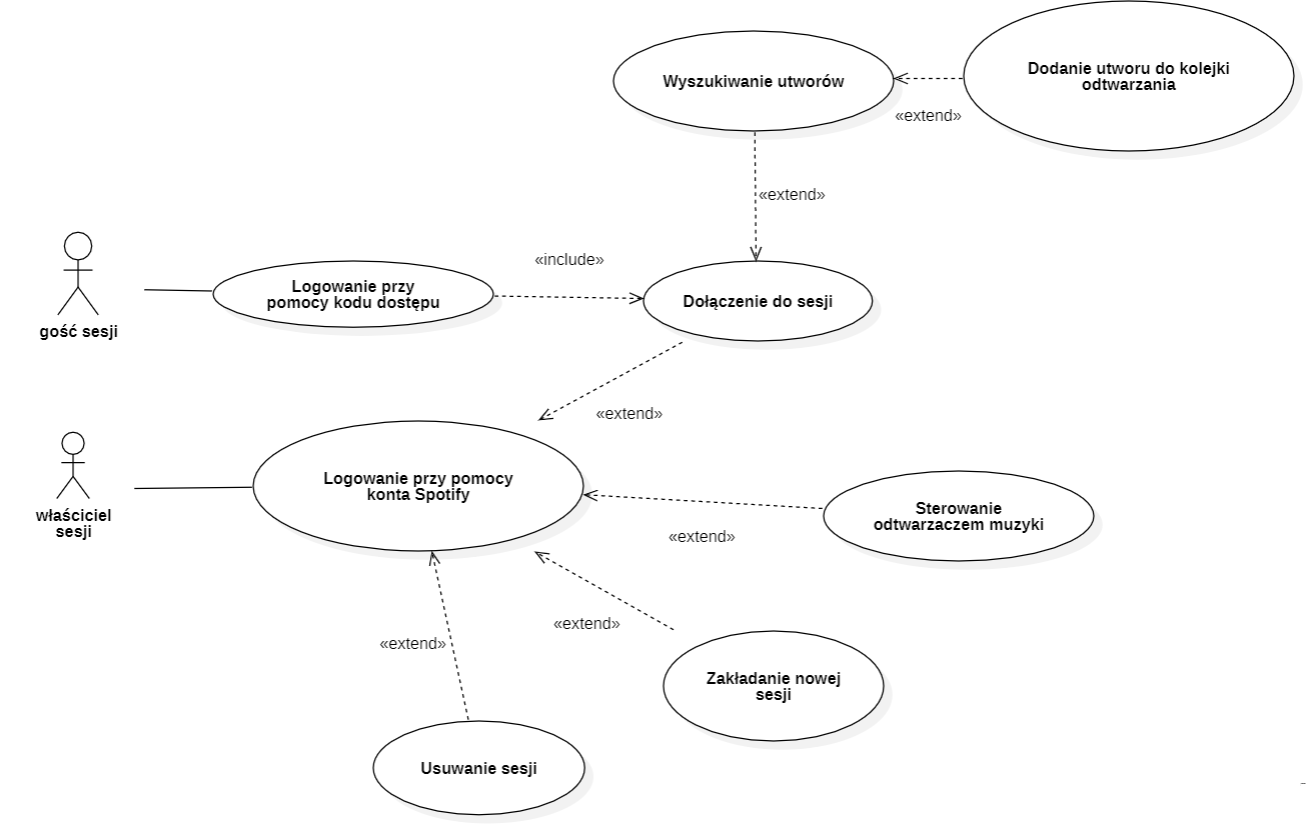
\includegraphics[width=0.95\textwidth]{./graf/przypadki_uzycia.PNG}
\caption{Przypadki użycia systemu}
\label{fig:use-case}
\end{figure}



\section{Opis narzędzi}

\subsection{Technologie serwera aplikacji (warstwa usług)}
Warunkami doboru technologii do wykonania części pracy działającej na serwerze była przede wszystkim uniwersalność oraz bezpieczeństwo aplikacji. Z tego powodu wybrany został język Java, który uruchamiany jest na wirtualnej maszynie (ang. \english{Java Virtual Machine}, JVM) wprowadzającej dodatkową warstwę abstrakcji między kodem Java a sprzętem komputerowym. JVM posiada wiele mechanizmów bezpieczeństwa (np. izolacja kodu czy automatyczne zarządzanie pamięcią) oraz umożliwia bezproblemowe uruchamianie programu na różnych platformach \cite{bib:java_virtual_machine}. Dużym atutem jest także ogromna społeczność programistów oraz bogaty ekosystem narzędzi oraz bibliotek, które można wykorzystać w projektach, co znacznie przyspiesza proces tworzenia oprogramowania.

Wraz z językiem Java użyta została platforma programistyczna Spring Boot \cite{bib:spring_boot}, która znacznie ułatwia tworzenie aplikacji serwerowych, przez dostarczanie gotowych rozwiązań oraz domyślne konfiguracje. Dużym atutem jest także modularność - architektura opiera się na mikro-serwisach, które pozwalają na dzielenie aplikacji na mniejsze części, co znacznie ułatwia skalowanie oraz dalszy rozwój aplikacji. Obecnie do tworzenia oprogramowania w Javie, Spring Boot jest najczęściej wybieraną platformą programistyczną \cite{bib:spring_market_analysis}.

Aby usprawnić implementację warstwy bazy danych, użyty został moduł Spring Data JPA \cite{bib:spring_jpa}, który umożliwia pominięcie pisania dużych ilości kodu SQL, ponieważ podstawowe operacje CRUD są automatycznie generowane. Programista tworząc klasę, która będzie odpowiedzialna za komunikację z bazą danych musi jedynie zaimplementować odpowiedni interfejs programistyczny. Dodatkowo umożliwia generowanie bardziej skomplikowanych zapytań wykorzystując do tego nazwę metody oraz mechanizm refleksji, w praktyce oznacza to, że pisanie jakiegokolwiek kodu SQL może się okazać zbędne. Spring Data JPA jest bardzo elastyczny i umożliwia korzystanie z różnych systemów bazodanowych oraz zapewnia automatyczne mapowanie obiektów Javy na tabele w~relacyjnej bazie danych (ang. \english{Object-Relational Mapping}, ORM).

Komunikacja z API Spotify została uproszczona przez użycie gotowego klienta \cite{bib:spotify_client_java}, który jest narzędziem programistycznym wprowadzającym dodatkową warstwę abstrakcji ukrywającą szczegóły komunikacji z zewnętrznym API, co ułatwia tworzenie oprogramowania i pozwala programiście skupić się na logice aplikacji.

\subsection{Technologie interfejsu użytkownika (warstwa prezentacji)}
Kluczowym aspektem w tworzeniu interfejsu użytkownika jest jego przejrzystość, intuicyjność oraz w jaki sposób aplikacja będzie zarządzać stanem. Dodatkowo, zgodnie z~założeniami projektu, system powinien być przystosowany do działania na urządzeniach mobilnych. Aby spełnić te wymogi do implementacji użyty został język TypeScript wraz z platformą programistyczną Angular \cite{bib:angular}, której głównym przeznaczeniem jest tworzenie jednostronicowych aplikacji internetowych (ang. \english{Single Page Application}, SPA). Dużą zaletą takiego rozwiązania jest pozbycie się konieczności przeładowywania zawartości strony w trakcie użytkowania aplikacji - zwiększa to interaktywność oraz efektywniej wykorzystuje zasoby. Dodatkowym atutem jest modularność, co minimalizuje powtarzalność tworzonego kodu oraz asynchroniczność wywoływania zapytań, która pozwala użytkownikowi na dalsze korzystanie z aplikacji pomimo oczekiwania na odpowiedź serwera. Angular zapewnia także wsparcie dla przeglądarek internetowych na urządzeniach mobilnych.

Dodatkowo w projekcie użyta została biblioteka Angular Materials \cite{bib:angular_materials}, która udostępnia gotowe szablony komponentów takich, jak wyskakujące okienka czy gotowe elementy formularzy. Pozwala to przyśpieszyć pracę nad tworzeniem oprogramowania.

\subsection{Baza danych (warstwa danych)}
Do realizacji warstwy danych użyty został system zarządzania bazami danych PostgreSQL. Dużą zaletą tego rozwiązania jest wysoka niezawodność zapewniona przez między innymi system kontroli spójności. Dodatkowym atutem jest skalowalność, która pozwala na zastosowanie tego rozwiązania zarówno w małych jak i w dużych systemach. 

\subsection{Platformy i usługi zewnętrzne}
Aby zapewnić spójność między warstwą prezentacji a warstwą usług wykorzystany został generator kodu \cite{bib:openapi_generator}, który na podstawie utworzonego przez programistę pliku opisującego powstające API (punkty końcowe, sposób autoryzacji, przyjmowane oraz zwracane wartości, opis obiektów uczestniczących w~wymianie między serwerem a~klientem itp.) generuje interfejsy programistyczne, obiekty modelu aplikacji oraz serwisy wykonujące zapytania w docelowym kodzie i wybranej technologii (w tym przypadku Java-Spring Boot oraz TypeScript-Angular), można powiedzieć że tworzony jest szkielet aplikacji pozbawiony logiki. Rolą programisty jest implementacja tych interfejsów oraz zastosowanie gotowych serwisów w odpowiednich miejscach zarówno po stronie klienta jak i serwera. Takie rozwiązanie ułatwia wprowadzanie zmian w wymianie klient-serwer oraz usprawnia tworzenie oprogramowania.

W projekcie użyta została platforma Docker \cite{bib:docker}, która umożliwia konteneryzację oprogramowania, co oznacza uruchomienie aplikacji z gotowego obrazu (program wraz z zależnościami takimi jak biblioteki, pliki konfiguracyjne etc.) na wirtualnej maszynie, z~którą można się komunikować oraz dowolnie zarządzać. Platforma wykorzystana była do symulacji serwera bazy danych.

\subsection{Środowisko deweloperskie}
Do implementacji oraz rozwoju omawianego systemu zostało użyte środowisko IntelliJ IDEA, zapewniające wsparcie dla języka Java oraz umożliwiające korzystanie z wtyczek oraz rozszerzeń, które znacznie ułatwiają pracę programisty. Interfejs użytkownika został utworzony przy pomocy Visual Studio Code, który wspiera składnię HTML, CSS oraz TypeScript. % Wymagania i narzędzia

% TODO
\chapter{Specyfikacja zewnętrzna}
\label{ch:04}
\section{Wymagania sprzętowe i programowe}
Do działania aplikacji wymagany jest serwer, na którym uruchomiona będzie warstwa usługowa projektu. Bazując na przeprowadzonych testach wydajności działającej aplikacji można stwierdzić, że wykorzystanie zasobów jest niewielkie - średnio 300MB pamięci RAM, 60MB przestrzeni dyskowej oraz wykorzystanie procesora na poziomie 2\% (testy uruchamiane na procesorze Intel Core i5-8250U). Aplikacja wymaga stałego połączenia do Internetu aby poprawnie działać (komunikacja z zewnętrznym API Spotify) oraz urządzenie, na którym aplikacja będzie uruchomiona musi być kompatybilne z maszyną wirtualną Javy (JVM). Dodatkowo do uruchomienia oprogramowania wymagana jest Java w wersji co najmniej 21. Warstwa prezentacji także wymaga serwera HTTP, z którego pobierane będą potrzebne dla klienta pliki ze strukturą aplikacji oraz potrzebnymi skryptami. Dodatkowo system wymaga dostępu do silnika bazodanowego postgreSQL w wersji 16.1. Wszystkie elementy systemu mogą działać na jednym urządzeniu (serwer HTTP, API oraz bazy danych), bądź dowolnie rozłożone na kilka osobnych urządzeń.

Aby klient mógł korzystać z aplikacji wymagana jest przeglądarka internetowa na dowolnym urządzeniu wspierająca obsługę języka JavaScript, HTML5 oraz CSS3 oraz połączenie z serwerem.

\section{Sposób instalacji}
W celu instalacji należy pobrać skompilowane pliki projektu bądź skompilować je we własnym zakresie. Do kompilacji potrzebne będą następujące narzędzia: 
\begin{itemize}
\item Środowisko Java w wersji 21
\item Narzędzie Maven
\item Narzędzie wiersza poleceń Angular CLI (Command Line Interface)
\item Narzędzie Node Package Manager
\end{itemize}

Aby skompilować oprogramowanie warstwy usług należy uruchomić wiersz poleceń, odnaleźć plik pom.xml w plikach projektu i przejść do jego lokalizacji (folder "Backend"), a następnie wywołać następujące polecenie: 

\lstinline|mvn compile|


Warstwa interfejsu użytkownika kompilowana jest w analogiczny sposób. Należy uruchomić wiersz poleceń, odnaleźć ścieżkę projektu interfejsu użytkownika i przejść do głównego folderu (folder "Frontend"). Następnie należy wywołać polecenie

\lstinline|ng build|



\section{Sposób aktywacji}
Przed uruchomieniem systemu należy skonfigurować aplikację serwera. W folderze z projektem warstwy usług należy zlokalizować plik "application.properites", w którym znajdują się następujące właściwości, które należy ustawić:
\begin{itemize}
\item \lstinline|base.address| - adres serwera HTTP udostępniającego warstwę interfejsu użytkownika
\item \lstinline|qrcode.address.suffix| - przyrostek adresu, który zakodowany w formie kodu QR. Otrzymany adres w kodzie QR będzie złączeniem trzech elementów: adresu serwera HTTP (base.address), przyrostka (qrcode.address.suffix) oraz kodu dostępu do danej sesji.
\item \lstinline|spotify.authorize.callbackUrl.suffix| - przyrostek adresu dodany do adresu serwera HTTP, na który użytkownik będzie przekierowany po pomyślnej autoryzacji kontem Spotify.
\item \lstinline|spotify.client.id, spotify.client.secret| -  wartości wymagane do komunikacji z zewnętrznym API serwisu Spotify.
\item \lstinline|jwt.secret| - klucz do generowania tokenów do autoryzacji użytkowników.
\item \lstinline|jwt.token.expirationtime| - czas wyrażony w sekundach określający ważność tokenu dostępu.
\item \lstinline|spring.datasource.url| - adres serwera bazy danych.
\item \lstinline|spring.datasource.username| - login użytkownika serwera bazy danych.
\item \lstinline|spring.datasource.password| - hasło użytkownika serwera bazy danych.
\end{itemize}

Załączone zostały dwa pliki wsadowe ze skryptami uruchamiającymi serwer aplikacji oraz serwer udostępniający warstwę prezentacji w trybie deweloperskim. Możliwe jest także uruchomienie obu aplikacji z poziomu wiersza poleceń wywołując polecenie 
\lstinline|ng serve| z głównego folderu z projektem warstwy interfejsu użytkownika (folder "Frontend").
Uruchomienie aplikacji serwera wymaga odnalezienia w folderze projektu aplikacji serwera (folder "Backend") folderu "target", w którym powinny znajdować się skompilowane pliki programu. Z tej lokalizacji należy wywołać polecenie \lstinline|java -jar backend-0.0.1-SNAPSHOT.jar|

Aby system mógł działać poprawnie należy dodatkowo zarejestrować swoją aplikację na platformie Spotify Developer \cite{bib:spotify_api} - umożliwi to korzystanie z API serwisu. Należy także skonfigurować adres zwrotny taki sam jak w konfiguracji aplikacji serwera. Oraz przekopiować wygenerowane klucze (spotify.client.id, spotify.client.secret).

\section{Kategorie użytkowników}
W systemie istnieją dwie kategorie użytkowników:
\begin{itemize}
\item Właściciel sesji

Do tej kategorii należą użytkownicy, którzy zostali zweryfikowani za pomocą własnego konta Spotify. Mają oni możliwość zakładania, moderacji oraz usuwania własnych sesji.

\item Gość sesji

W tej kategorii znajdują się użytkownicy, którzy dostęp do systemu uzyskali poprzez użycie poprawnego kodu dostępu, bądź zeskanowanie kodu QR uzyskanych od właściciela sesji. Użytkownik ten może należeć tylko do jednej sesji, w przypadku której usunięcia jest likwidowany. Ma możliwość wyszukania utworów oraz dodania ich do kolejki, jeśli zostały spełnione warunki ustawione przez właściciela sesji.

\end{itemize}
\section{Sposób obsługi}
Aby skorzystać z systemu należy na dowolnej przeglądarce wpisać skonfigurowany adres URL a następnie postępować dalej z instrukcjami wyświetlonymi na ekranie. Aplikacja w obecnej chwili nie wspiera rozdzielczości ekranów urządzeń mobilnych więc niektóre elementy mogą być niewidoczne lub ciężko dostępne w pionowym układzie urządzenia.

Kod dostępu do sesji jest dostępny w widoku sesji, u góry obok nazwy (Rys. \ref{fig:session-menu-owner}, natomiast wygenerowany kod QR zostaje wyświetlony po użyciu przycisku "TV mode" dostępnego przy pasku do zarządzania odtwarzaniem muzyki.

\section{Administracja serwerem}
Możliwa jest ingerencja poprzez użycie systemu do zarządzania bazą danych. Przykładowo usunięcie użytkownika z odpowiedniej tabeli odbierze mu uzyskany dostęp do systemu i wymusi ponowną autoryzację. Dodatkowo, gdy aplikacja w serwisie Spotify jest zarejestrowana w trybie deweloperskim, użytkownik może zakładać sesję oraz korzystać z systemu jedynie po udzieleniu mu dostępu przez panel administratora udostępniony przez platformę Spotify.

\section{Kwestie bezpieczeństwa}
W celu uwierzytelnienia użytkowników użyty został standard JWT (JSON Web Token), który definiuje format bezpiecznego oraz niezmiennego sposobu przesyłania informacji. Token to zaszyfrowany ciąg znaków składający się z trzech części: 
\begin{itemize}
\item Nagłówek - określa typ tokenu oraz sposób szyfrowania
\item Dane - zawiera informacje o użytkowniku takie jak kategoria, czy identyfikator oraz informacje o dacie wygaśnięcia tokenu
\item Podpis - jest to część utworzona na podstawie nagłówka oraz ładunku, jego celem jest zapewnienie integralności danych i uwierzytelnienia źródła.
\end{itemize}

Token zostaje udostępniony użytkownikowi w momencie, gdy jego tożsamość zostanie potwierdzona (poprzez wprowadzenie poprawnego kodu dostępu do sesji lub pomyślną autoryzację konta Spotify). Bez odpowiedniego tokenu użytkownik nie ma dostępu do żadnej funkcjonalności systemu z wyjątkiem możliwości uwierzytelnienia. Dodatkowo niektóre funkcje są dostępne tylko dla użytkowników odpowiedniej kategorii - przykładowo gość nie ma możliwości sterowania odtwarzaczem muzyki. Generacja tokenu wykorzystuje klucz, który nie może być udostępniony poza serwerem, należy więc w pliku konfiguracyjnym serwera wygenerować oraz ustawić własny klucz (pole jwt.secret)

Aby zapewnić bezpieczeństwo kont Spotify użytkowników, odpowiednie tokeny umożliwiające dostęp do zewnętrznego API Spotify, identyfikujące użytkownika, są przechowywane w bazie danych i nigdy nie są przekazywane bezpośrednio do klientów. Zamiast tego, wykorzystywane są do komunikacji z API, a otrzymane wyniki są zwracane do klienta przez warstwę usług systemu co uniemożliwia przechwycenie i ingerencję przez osoby trzecie w konta Spotify użytkowników.

Kody dostępu do sesji są generowane losowo i składają się z 6 znaków (wszystkie cyfry oraz litery alfabetu łacińskiego bez rozróżnienia na wielkości liter). Zastosowanie takiego mechanizmu znacząco utrudnia próbę zgadnięcia kodu i zwiększa ochronę przed atakami typu brute-force, ponieważ liczba wszystkich kombinacji wynosi $36^6$, czyli ponad 2 miliardy.

\section{Przykład działania}
Przypuśćmy, że na wydarzeniu towarzyskim powinna być odtwarzana w tle muzyka. Użytkownik decyduje się skorzystać z systemu więc wpisuje adres w przeglądarkę i loguje się używając swojego konta Spotify. Następnie zostaje przeniesiony do menu, gdzie może utworzyć nową sesję lub uruchomić własną już istniejącą. Użytkownik następnie uruchamia odtwarzanie muzyki używając do tego na przykład dedykowanej aplikacji Spotify i udostępnia wszystkim uczestnikom wydarzenia kod dostępu. Uczestnicy otwierają aplikację na swoich urządzeniach gdzie, mogą dołączyć do sesji korzystając z kodu. Po pomyślnej autoryzacji użytkownicy zostają przeniesieni do menu gdzie, mogą wyszukać oraz dodać utwory do kolejki odtwarzania, sprawdzić jakie utwory są następne w kolejce oraz kto jest uczestnikiem sesji. Dodatkowo, jeśli właściciel nie zablokował tej funkcji na koncie Spotify właściciela sesji tworzona jest publiczna playlista, dostęp do której posiada każdy gość w sesji.

\section{Scenariusze korzystania z systemu}
\subsection{Zakładanie oraz dołączanie do sesji}

\begin{enumerate}
\item Przypadek użycia rozpoczyna się gdy użytkownik uruchomi aplikację w przeglądarce internetowej.
\item Użytkownik wybiera z menu opcję zakładania sesji (Rys. \ref{fig:auth-menu}).
\begin{figure}[h]
\centering
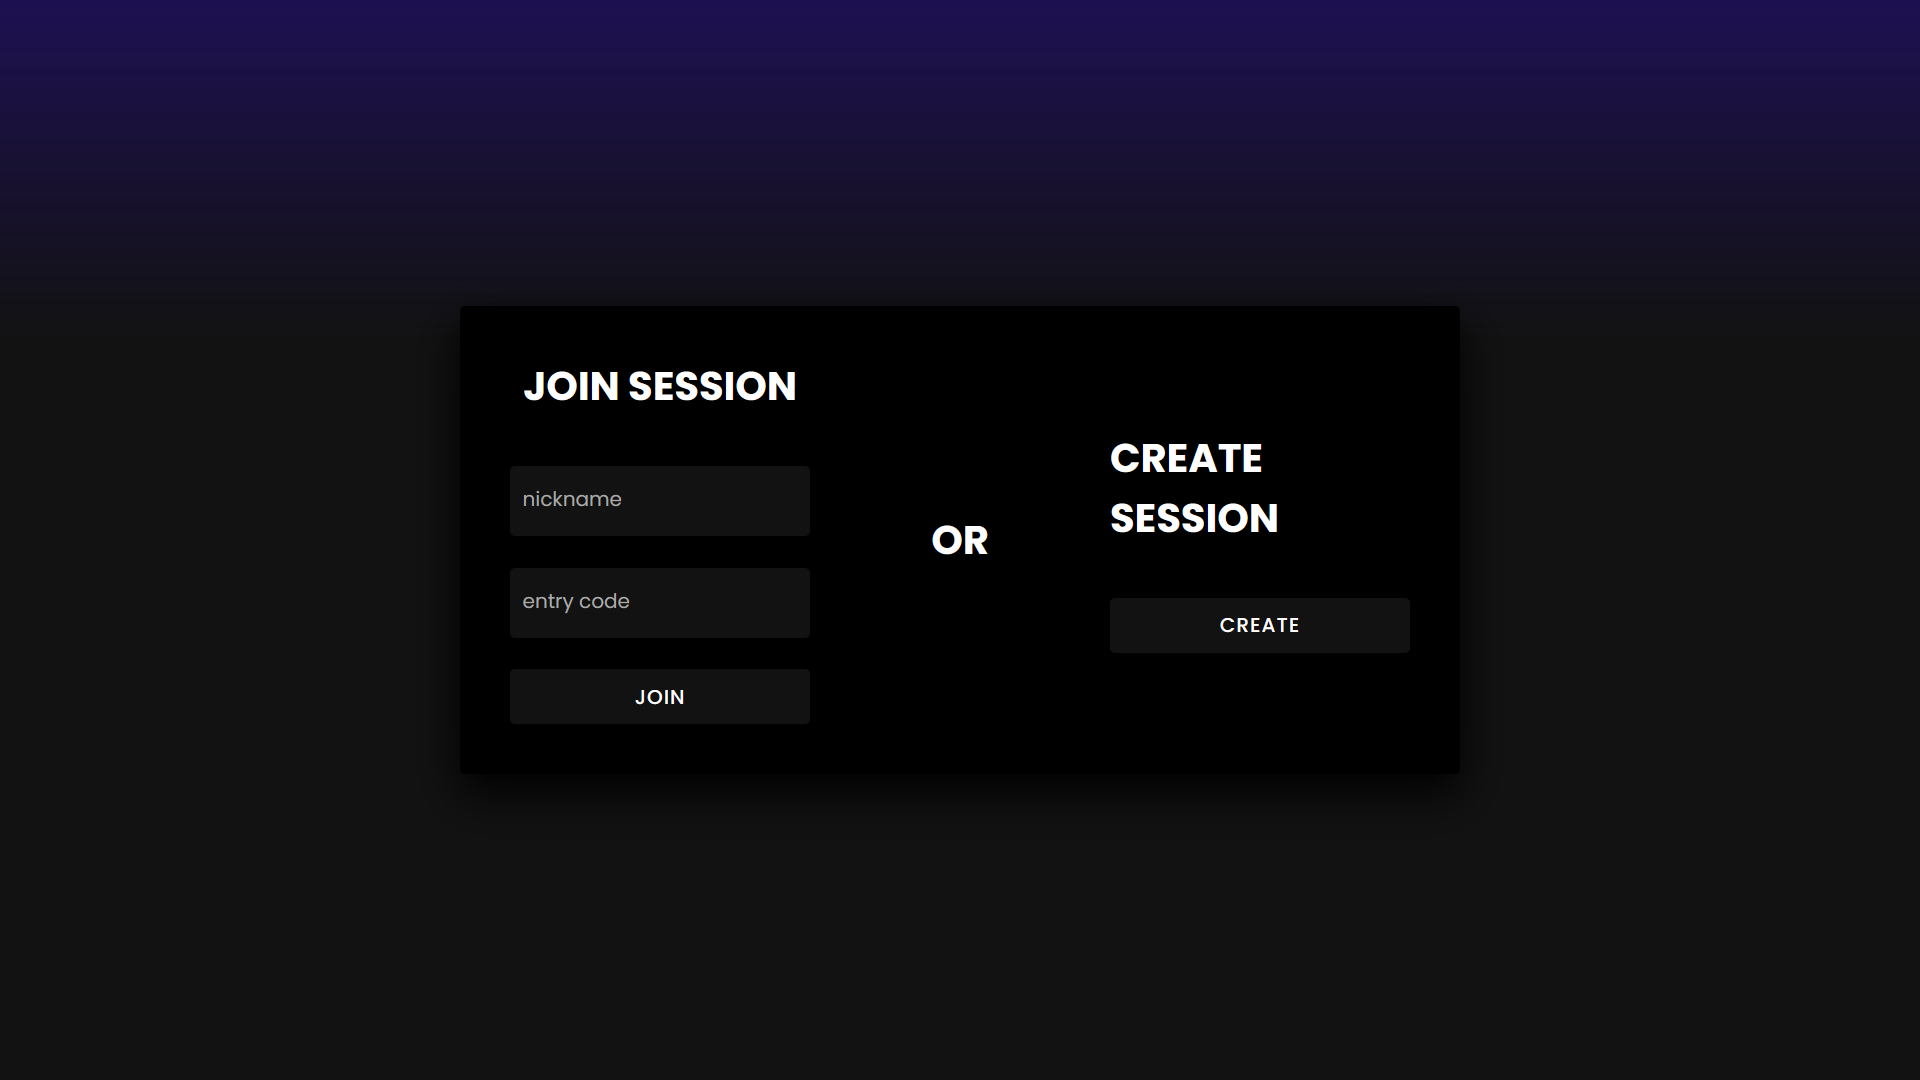
\includegraphics[width=0.95\textwidth]{./graf/auth_menu.png}
\caption{Wygląd interfejsu użytkownika - główne menu logowania}
\label{fig:auth-menu}
\end{figure}

\item Użytkownik jest przeniesiony na stronę autoryzacji Spotify, gdzie ma możliwość zalogowania się do swojego konta oraz proszony jest o wyrażenie zgody na określone warunki (Rys. \ref{fig:spotify-menu}).
\begin{figure}[h]
\centering
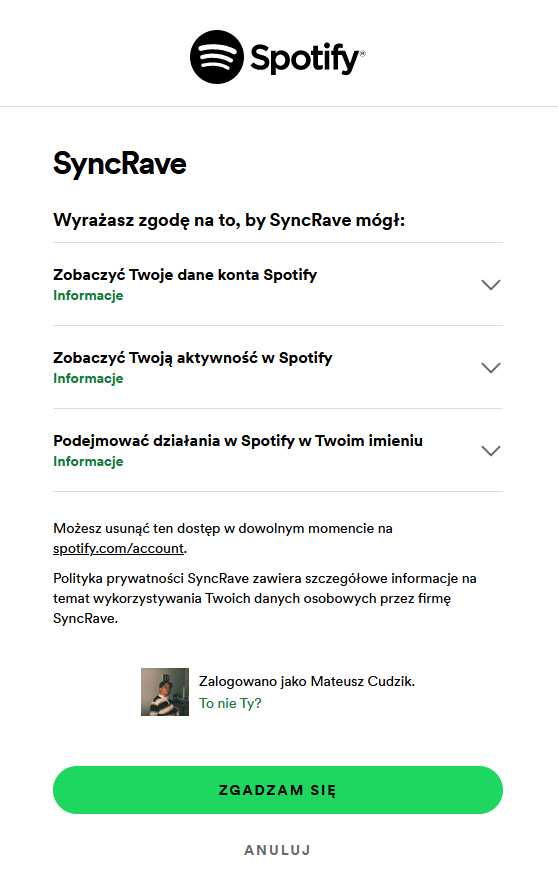
\includegraphics[width=0.95\textwidth]{./graf/spotify_permission.PNG}
\caption{Wygląd interfejsu użytkownika - menu wyrażenia zgody w serwisie Spotify}
\label{fig:spotify-menu}
\end{figure}

\item System przenosi użytkownika do menu gdzie udostępniony jest formularz zakładania sesji (Rys. \ref{fig:admin-menu}).
\begin{figure}[h]
\centering
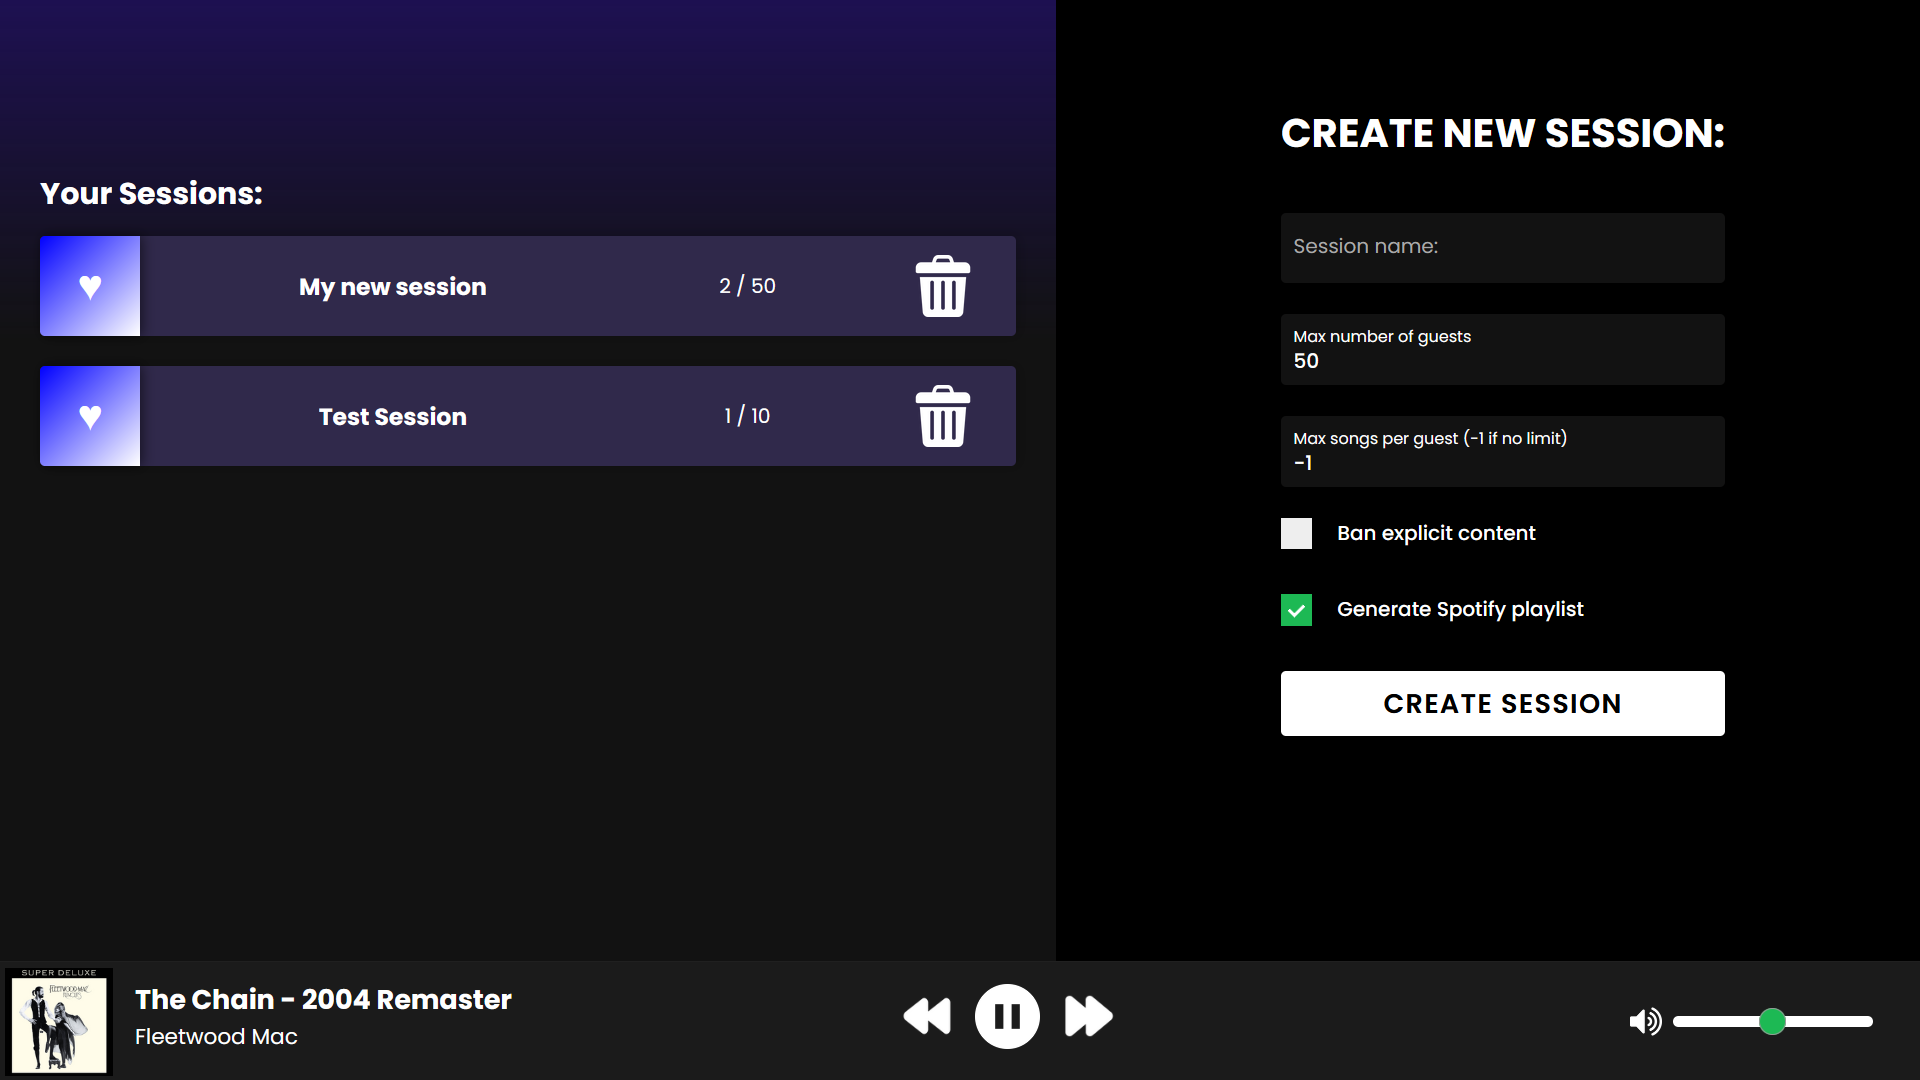
\includegraphics[width=0.95\textwidth]{./graf/admin_menu.png}
\caption{Wygląd interfejsu użytkownika - główne menu właściciela sesji}
\label{fig:admin-menu}
\end{figure}

\item Po wypełnieniu i zatwierdzeniu przez użytkownika formularza, system sprawdza poprawność wypełnionych danych.
\item Dodana sesja pojawia się z lewej strony menu właściciela sesji.
\item Jeśli użytkownik zdecyduje się dołączyć do jednej z sesji wybiera ją z listy.
\item System przenosi użytkownika do widoku sesji w wersji właściciela (Rys. \ref{fig:session-menu-owner}).
\begin{figure}[h]
\centering
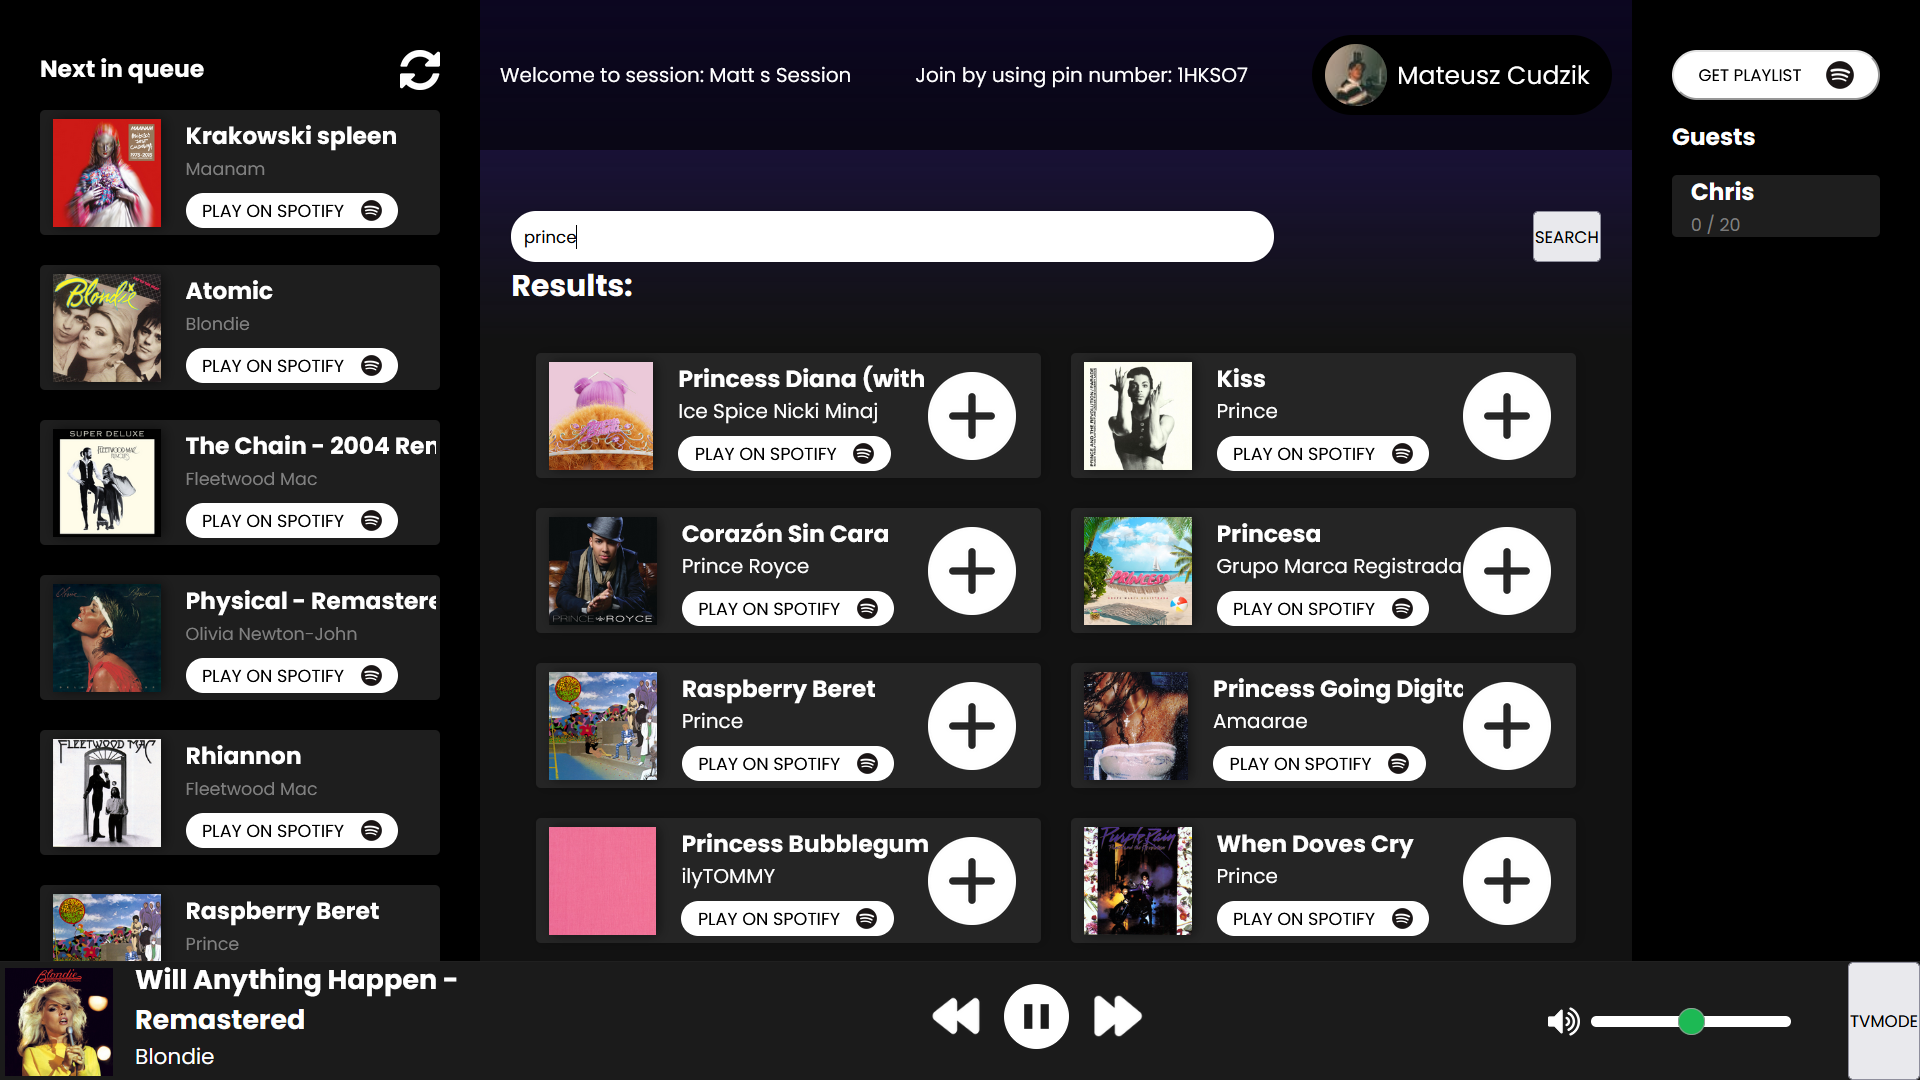
\includegraphics[width=0.95\textwidth]{./graf/admin_session_menu.png}
\caption{Wygląd interfejsu użytkownika - widok sesji w wersji właściciela}
\label{fig:session-menu-owner}
\end{figure}
\end{enumerate}

\subsection{Dołączenie do istniejącej sesji}
\begin{enumerate}
\item Przypadek rozpoczyna się, gdy użytkownik uruchomi aplikację w przeglądarce internetowej przez wpisanie poprawnego adresu lub zeskanowanie kodu QR z adresem.
\item System wyświetla użytkownikowi menu (Rys. \ref{fig:auth-menu}), w którym proszony jest o wpisanie pseudonimu, którym będzie się posługiwał oraz kodu dostępu do sesji. W przypadku gdy użytkownik zeskanował kod QR kod dostępu będzie automatycznie wpisany w odpowiednie pole.
\item Po zatwierdzeniu formularza system sprawdza poprawność danych.
\item Użytkownik przeniesiony jest do menu widoku sesji w wersji gościa (Rys. \ref{fig:session-menu-guest}). Przypadek użycia się kończy.
\begin{figure}[h]
\centering
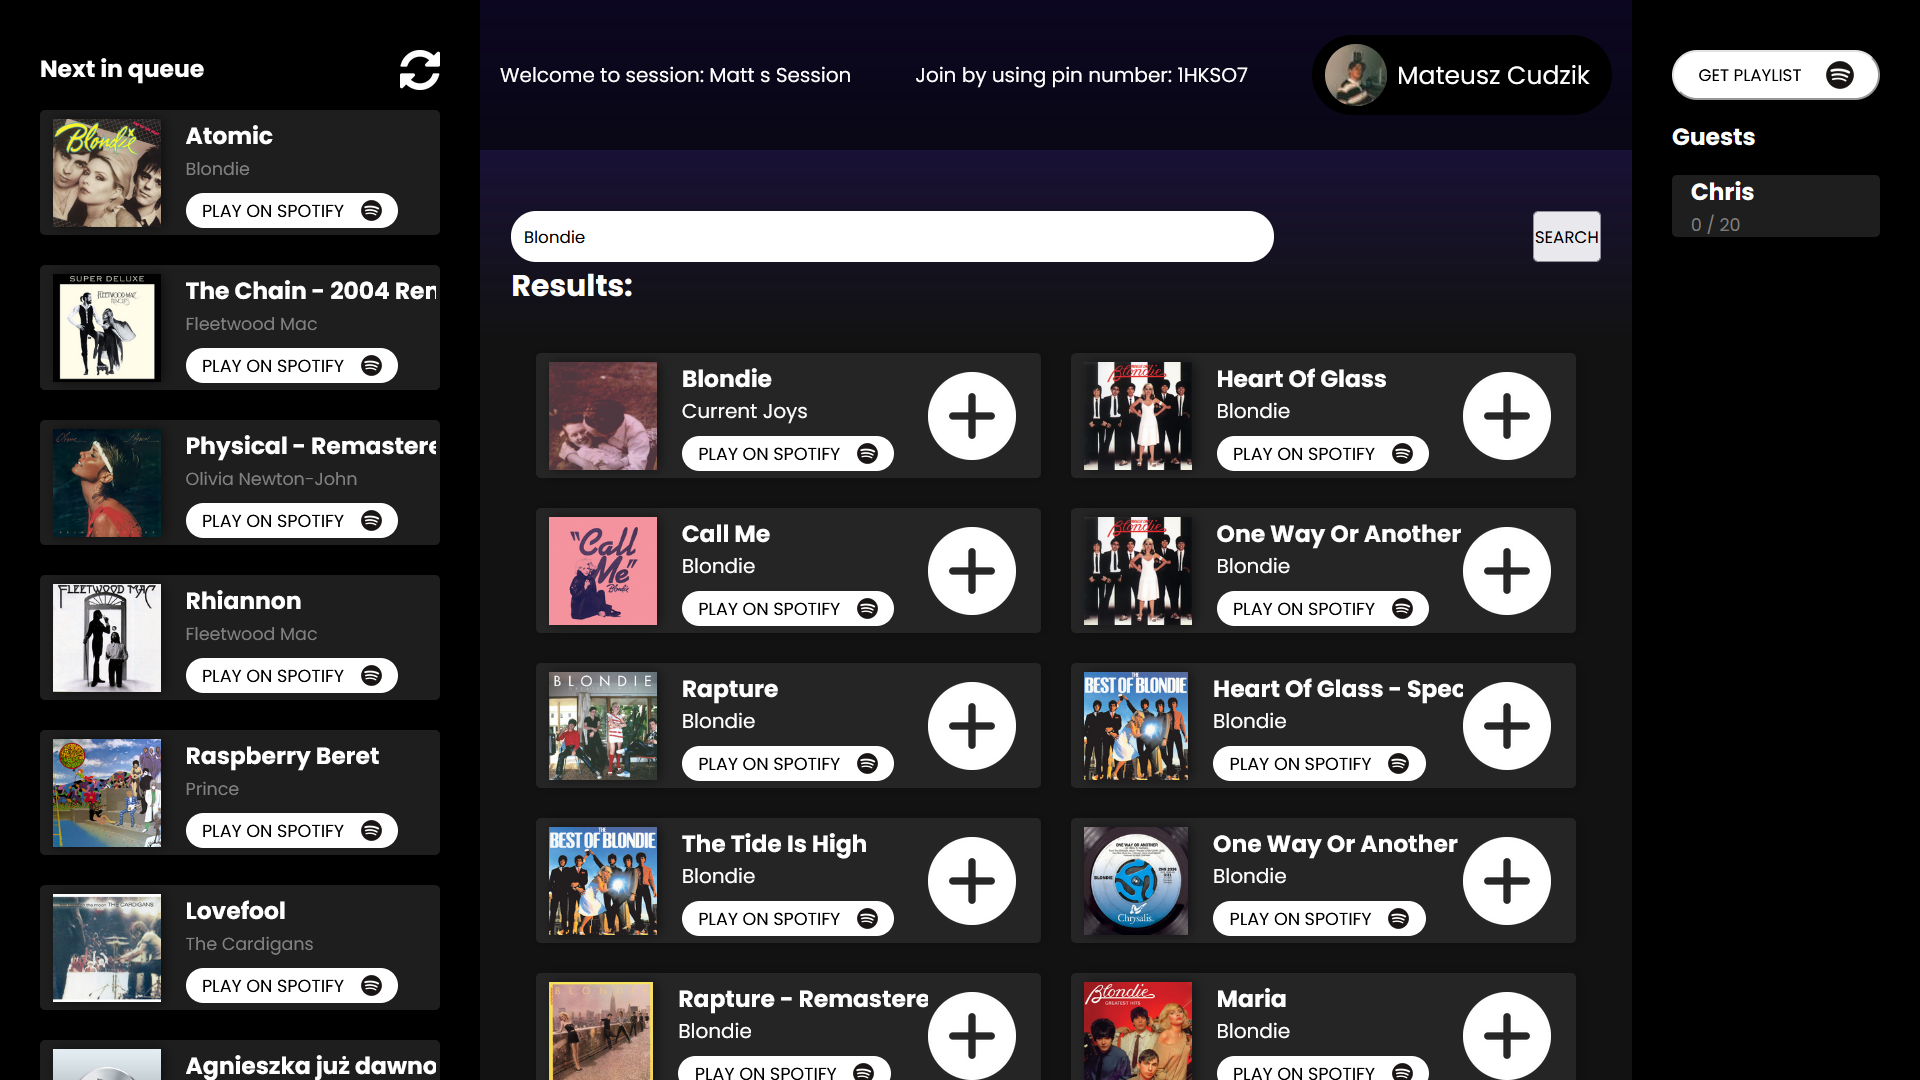
\includegraphics[width=0.95\textwidth]{./graf/guest_session_menu.PNG}
\caption{Wygląd interfejsu użytkownika - widok sesji w wersji gościa}
\label{fig:session-menu-guest}
\end{figure}
\end{enumerate}

\subsection{Dodawanie utworu do kolejki}
\begin{enumerate}
\item Przypadek rozpoczyna się gdy użytkownik znajduje się w menu widoku sesji Rys. \ref{fig:session-menu-guest} lub Rys. \ref{fig:session-menu-owner}.
\item Użytkownik wpisuje w pole wyszukiwania odpowiednią frazę. Może to być artysta, tytuł utworu lub albumu.
\item Po zatwierdzeniu system zwraca wyniki wyszukiwania.
\item Użytkownik może dodać znaleziony utwór używając odpowiedniego przycisku obok wyniku.
\item Jeśli utwór spełnia zasady sesji oraz użytkownik nie osiągnął limitu utwór zostaje dodany na koniec kolejki. Limity te nie dotyczą właściciela sesji. Przypadek użycia się kończy.
\end{enumerate}

 % [Właściwy dla kierunku -- np. Specyfikacja zewnętrzna]

% TODO
\chapter{Specyfikacja wewnętrzna}
\label{ch:05}

\section{Przedstawienie idei}
Celem aplikacji, jest umożliwienie wielu użytkownikom wspólnego zarządzania listą odtwarzania utworów. Aby to osiągnąć wykorzystane zostało API serwisu Spotify, które umożliwia ingerencję w konto użytkownika, który wyraził na to zgodę (logując się do systemu). Dzięki udostępnionym funkcjom aplikacja ma dostęp do bazy utworów serwisu, możliwe jest także sterowanie odtwarzaczem muzyki, w tym dodawanie utworów do kolejki odtwarzania. Po poprawnym zalogowaniu przez użytkownika Spotify system zapisuje w bazie jego tokeny umożliwiające dostęp do zapytań, które ingerują w jego konto. W momencie, kiedy gość sesji doda utwór do kolejki, aplikacja serwera używając odpowiednich tokenów dodaje utwór w imieniu właściciela.

Aby zapewnić prostotę używania aplikacji, system nie wymaga od gości sesji rejestracji, a jedynie podania poprawnego kodu oraz pseudonimu. Serwer w odpowiedzi na udaną autoryzację odsyła token dostępu, bez którego wszystkie zapytania, które nie należą do punktu końcowego autoryzacji zostaną odrzucone. Tokeny dostępu mają datę ważności, po której przestają działać a konto zostaje dezaktywowane, użytkownik musi się wtedy ponownie uwierzytelnić.


\section{Architektura systemu}
Zgodnie z wielowarstwowym modelem aplikacji internetowej system składa się z 3 osobnych elementów:
\subsection{Warstwa danych}
Warstwa odpowiedzialna za przetrzymywanie oraz pozyskiwanie danych została zrealizowana przy pomocy gotowych już narzędzi. Serwer, na którym działa silnik bazy danych (PostgreSQL) obsługuje zapytania SQL. W trakcie implementacji serwer bazy danych został utworzony lokalnie na maszynie wirtualnej przy pomocy narzędzia Docker. Interakcję z bazą danych implementuje mechanizm dostępny jako moduł szkieletu Spring. Udostępnia on przejrzysty i łatwy w obsłudze interfejs programistyczny, który wprowadza pewną warstwę abstrakcji, aby ułatwić realizację interakcji z bazą danych.

\subsection{Warstwa usług}
Część systemu realizująca logikę biznesową została zaimplementowana korzystając ze szkieletu programistycznego Spring oraz języka Java. Aplikacja implementuje architekturę opartą na wzorcu model-widok-kontroler, natomiast warstwa widoku została zrealizowana w osobnej aplikacji. Dodatkowo istnieje jeszcze warstwa zapewniająca bezpieczeństwo systemu.

Po otrzymaniu zapytania przez serwer trafia ono do łańcucha filtrów, które sekwencyjnie sprawdzają żądanie między innymi w celach bezpieczeństwa. W aplikacji zaimplementowane zostały dwa filtry, które sprawdzają tożsamość użytkownika (uwierzytelnianie) na podstawie tokenu JWT obecnego w nagłówku żądania. Kolejnym etapem jest autoryzacja, czyli potwierdzenie czy uwierzytelniony użytkownik ma dostęp do zasobu, którego żąda. Następnie żądanie jest mapowane do odpowiedniego kontrolera, który wywołuje odpowiednie serwisy implementujące logikę biznesową. Serwisy korzystają z repozytoriów, których głównym zadaniem jest komunikacja z bazą danych. Dodatkowo wykorzystują inne serwisy, które przykładowo realizują połączenie z zewnętrznym API platformy Spotify. Otrzymane wyniki są odpowiednio przetwarzane przez serwisy i zwracane do kontrolera, który odsyła odpowiedź do klienta. Serwisy stanowią część modelu aplikacji.

\subsection{Warstwa prezentacji}
Jest to część systemu odpowiedzialna za interakcję z użytkownikiem, została zaimplementowana przy użyciu szkieletu programistycznego Angular oraz języka TypeScript. Aplikacja została utworzona w architekturze SPA co oznacza, że aplikacja raz pobrana z serwera WWW nie wymaga przeładowania w celu zmiany wyświetlanych treści, lecz jest to wykonywane asynchronicznie w tle. Aplikacja składa się z komponentów, które reprezentują każdą część interfejsu użytkownika i realizują daną funkcjonalność oraz określają styl i rozmieszczenie poszczególnych elementów. Przykładowo komponent, który implementuje funkcjonalność odtwarzacza muzyki, może być ponownie używany w innych komponentach bez konieczności niepotrzebnego powtarzania kodu. Komponenty korzystają z serwisów, których zadaniem jest komunikacja z warstwą usług. Serwisy udostępniają funkcje, które odpowiednio tworzą, wysyłają oraz odbierają zapytania. Obiekty, które uczestniczą w wymianie między warstwą prezentacji a warstwą usług są zdefiniowane w modelu aplikacji.

\section{Organizacja bazy danych}
Aby zrealizować założenia projektu konieczne było zaprojektowanie oraz implementacja bazy danych. Diagram przedstawiony na Rys. \ref{fig:database} pokazuje jakie relacje zachodzą między poszczególnymi tabelami. W centrum diagramu widnieje kluczowy element systemu - sesja, przechowuje ona podstawowe informacje takie jak data utworzenia czy kod dostępu oraz nazwę. Sesja jest ściśle powiązana z tabelą właścicieli, gdzie właściciel może posiadać wiele sesji natomiast sesja tylko jednego właściciela. Tabela właścicieli przechowuje informacje niezbędne do komunikacji z zewnętrznym API platformy Spotify - tokeny dostęp oraz nazwę i id użytkownika w serwisie. Ustalone zasady sesji są unikatowe dla każdej sesji i przechowują informację o ustalonych przez właściciela wartościach takich jak maksymalna ilość utworów, które może dodać gość czy maksymalna ilość gości w sesji oraz czy dozwolone będą utwory oznaczone jako zawierające treści dla dorosłych i czy powinna zostać utworzona lista z dodanymi utworami. W bazie danych przetrzymywane są także informacje o gościach, którzy dołączyli do sesji takie jak ilość dodanych przez nich utworów oraz pseudonim, który ustawili dołączając do sesji. Gość może należeć tylko do jednej sesji, natomiast w sesji może znajdować się wielu gości. Baza danych zawiera także informacje o tym jakie utwory zostały dodane do kolejki w danej sesji oraz jakie gatunki utworów właściciel zablokował, funkcjonalność ta jest obecnie dostępna jedynie z poziomu API aplikacji i nie jest możliwa do ustawienia używając interfejsu użytkownika.


\section{Użyte biblioteki}
\begin{itemize}
\item Lombok - biblioteka generująca powtarzalny i rutynowy kod taki jak konstruktor czy metody pobierające i ustawiające wartości obiektu poprzez użycie odpowiednich adnotacji, co poprawia czytelność kodu. 

\item io.jsonwebtoken - biblioteka obsługująca tokeny JWT, za pomocą której możliwe jest tworzenie, walidacja oraz parsowanie tokenów dostępu.

\item ZXing - biblioteka umożliwiająca generowanie kodów QR.

\item Jakarta Bean Validation - narzędzie służące do walidacji danych, poprzez odpowiednie adnotacje, dzięki czemu reguły dotyczące pól obiektów są wyraźnie zdefiniowane.

\item ngx-cookie-service - moduł biblioteki obsługującej pliki cookie, w których trzymany jest token dostępu po autoryzacji użytkownika.
\end{itemize}

\section{Ważniejsze klasy}
\begin{itemize}
\item Interfejsy kontrolerów API

Są to automatycznie wygenerowane klasy przez narzędzie OpenAPI generator. Tworzą one szkielet aplikacji i definiują sygnatury metod, które należy zaimplementować. Każda z funkcji opatrzona jest odpowiednimi adnotacjami, które określają ścieżkę, parametry oraz ich walidację, metody autoryzacji, rodzaj żądania odpowiadającemu danemu punktowi końcowymi itp.

\item Serwisy

Klasy implementujące logikę biznesową korzystając z innych serwisów oraz bazy danych poprzez metody udostępniane przez repozytoria. Każda klasa implementuje odpowiedni interfejs aby zapewnić niezależność między deklaracją metod a ich implementacją. Większość serwisów dodatkowo mapuje otrzymane wyniki na obiekty, które uczestniczą w komunikacji z klientem.

\item Klasa do generacji kodów dostępu i kodów QR

Generowanie nowych kodów dostępu odbywa się podczas tworzenia nowych sesji. Na Rys. \ref{fig:code-generation} przedstawiony jest kod, który jest za to odpowiedzialny. Z tablicy dozwolonych znaków w sposób losowy wybrane jest kolejno 6 znaków. Kluczowa tutaj jest klasa SecureRandom, która jest dużo bardziej bezpieczna pod względem kryptografii. Do generacji liczby losowej wykorzystane jest kilka źródeł losowości takich jak ruch sieciowy, ruch dyskowy czy czas systemowy. 

\begin{figure}[h]
\centering
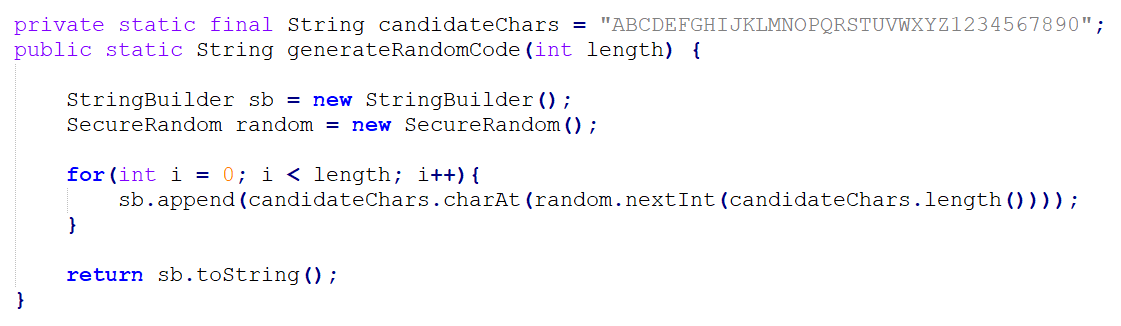
\includegraphics[width=0.9\textwidth]{./graf/code_generation.PNG}
\caption{Fragment kodu - generowanie losowych kodów dostępu}
\label{fig:code-generation}
\end{figure}

\end{itemize}
\section{Szczegóły implementacji}
\subsection{Zastosowane wzorce projektowe}
\begin{itemize}
\item Pełnomocnik

Aby zapewnić kontrolę dostępu do danych z serwisu Spotify oraz dalszą ich modyfikację i korzystanie z nich w logice biznesowej zastosowany został wzorzec pełnomocnika. Oznacza to, że otrzymane wyniki zanim zostaną zwrócone do klienta są dodatkowo modyfikowane i używane w implementacji logiki, aby przykładowo sprawdzić czy utwór, który użytkownik chciał dodać spełnia zasady sesji. Dodatkowo chronione są dzięki temu dane użytkowników Spotify, ponieważ ich tokeny dające dostęp do niektórych funkcjonalności konta w serwisie nie są nigdy udostępniane na zewnątrz.

\item Model-Widok-Kontroler

Zastosowany został podział, który rozdziela logikę od wyglądu w systemie, zapewniając jednocześnie niezależność obu komponentów co pozwala dowolnie zmieniać ich sposób realizacji. Komunikację między modelem a widokiem zapewnia kontroler.

\item Architektura wielowarstwowa (dokładnie trójwarstwowa)

Zastosowany został podział, dzielący system na trzy warstwy: prezentację, czyli interfejs użytkownika, logikę biznesową oraz dane. Każdy z wymienionych modułów to osobna aplikacja, dzięki czemu zachowana jest niezależność.

\item Wstrzykiwanie zależności

Mechanizmy szkieletu programistycznego Spring implementują ten wzorzec, aby przekazywać zależności między obiektami w prosty sposób bez konieczności ingerencji w przekazywany komponent. Zależności są dostarczane do obiektu co poprawia łatwość utrzymania aplikacji.
\end{itemize}
\section{Diagramy UML}

\begin{figure}[h]
\centering
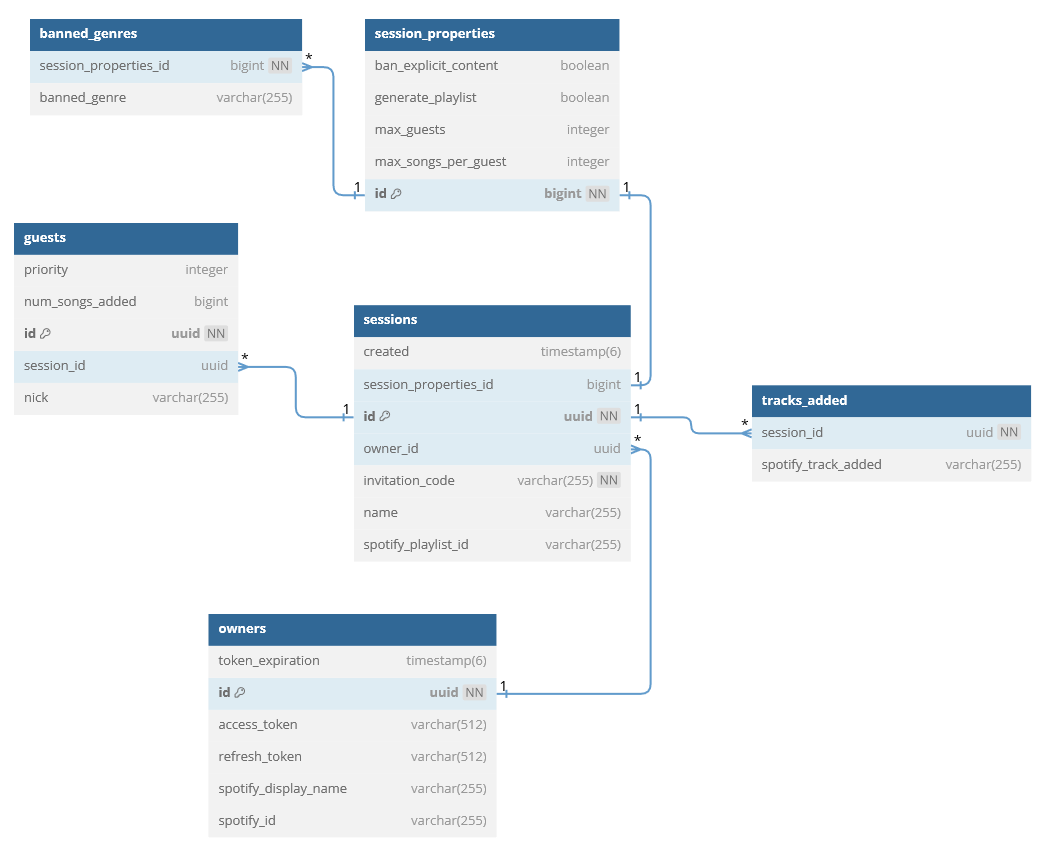
\includegraphics[width=1.0\textwidth]{./graf/database_diagram.png}
\caption{Diagram modelu bazy danych}
\label{fig:database}
\end{figure}



 % [Właściwy dla kierunku -- np. Specyfikacja wewnętrzna]

% TODO
\chapter{Weryfikacja i walidacja}
\label{ch:06}
\section{Sposób testowania w ramach pracy}
Podczas rozwoju systemu na bieżąco były wykonywane testy integracyjne oraz testy jednostkowe mające na celu walidację poprawności działania zaimplementowanych komponentów. 

Dodatkowo przeprowadzony został test wydajnościowy, w którym zmierzona została ilość użytej pamięci RAM przez uruchomioną aplikację, do której trafiały 4 różne zapytania co 20ms. Wyniki zaprezentowane na rys. \ref{fig:performance} pokazują, że aplikacja najwięcej zasobów zużyła podczas uruchomienia, a w ciągu normalnego działania zużywane są niewielkie ilości - zużycie procesora na poziomie 2\% oraz wykorzystanie pamięci 
\begin{figure}[h]
\centering
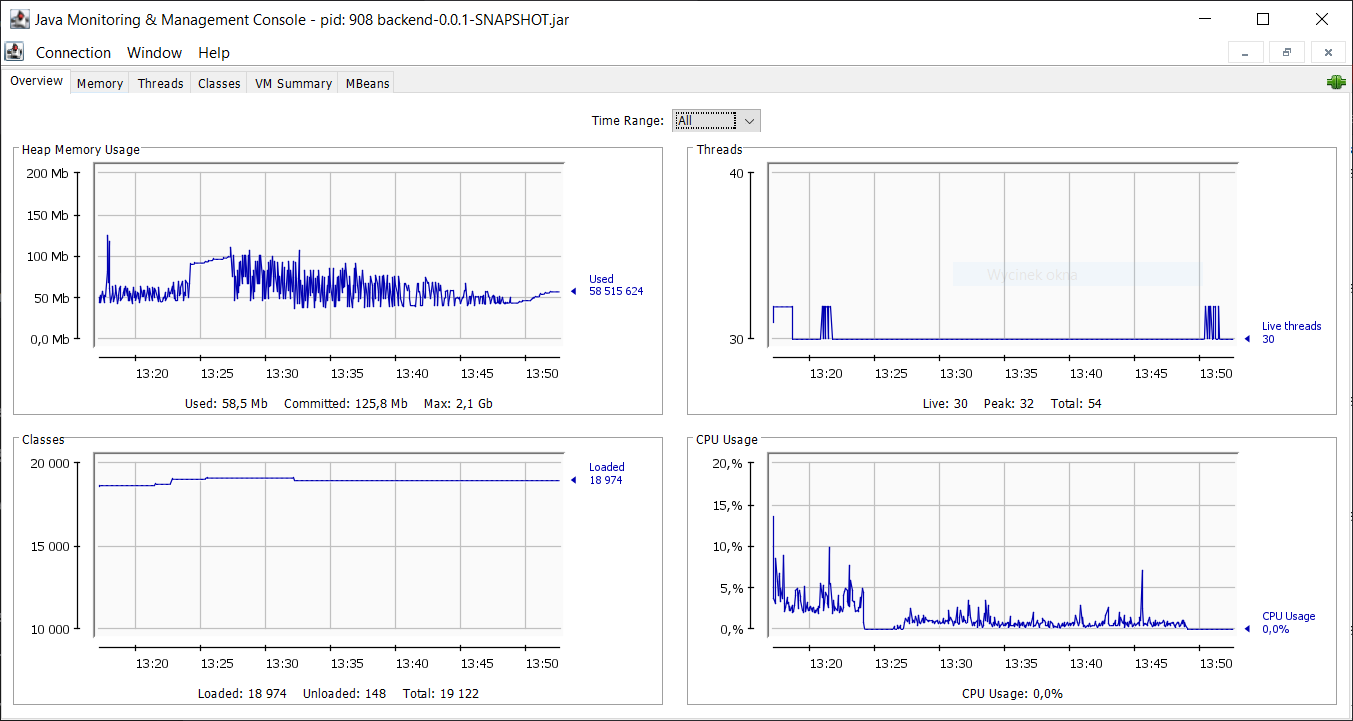
\includegraphics[width=0.95\textwidth]{./graf/performance.PNG}
\caption{Wyniki testu wydajnościowego}
\label{fig:performance}
\end{figure}

\section{Organizacja eksperymentów}
Aby przeprowadzić testy użyte zostało narzędzie Postman, które umożliwia tworzenie oraz wysyłanie żądań HTTP do serwera z ustawionymi danymi, nagłówkami oraz parametrami i~pozwala odczytać otrzymane wyniki. Narzędzie to pozwoliło na bieżące testy API bez konieczności implementacji interfejsu użytkownika. Platforma została także użyta w teście wydajnościowym, aby symulować ruch w sieci.

Pomiary wydajnościowe zostały wykonane przy użyciu konsoli monitorowania i~zarządzania w Javie, która umożliwia monitorowanie aplikacji oraz zbieranie danych diagnostycznych. 

Dodatkowo podczas implementacji interfejsu użytkownika, wykorzystane zostało narzędzie inspektora dostępne w przeglądarce internetowej.

\section{Przypadki testowe, zakres testowania}
W aplikacji serwera przetestowane zostały wszystkie punkty końcowe pod względem poprawności przyjmowanych danych (niepoprawna długość, niedozwolone znaki, puste lub wypełnione białymi znakami łańcuchy znaków itp.), dodatkowo sprawdzone zostało czy zapytania, które odnoszą się do nieistniejących danych są poprawnie odrzucane (nieistniejące sesje, użytkownicy itp.). Punkty końcowe aplikacji serwera zostały przetestowane także pod względem bezpieczeństwa - nieważny token bezpieczeństwa lub jego całkowity brak czy próby dostępu do niedozwolonych dla danej kategorii użytkowników funkcji takiej, jak sterowanie odtwarzaczem muzyki przez gościa sesji. Przetestowana została także poprawność działania zasad sesji, które blokują użytkownikom dodawanie utworów ponad ustawiony limit czy dołączanie do sesji, która jest już pełna.

\section{Wykryte i usunięte błędy}
Podczas implementacji systemu wykryto oraz usunięto stosunkowo dużo błędów, najczęściej występowały w kodzie aplikacji serwera. Przykładem może być błąd, który powodował odrzucanie wszystkich zapytań pochodzących z aplikacji klienta przez serwer. Błąd nie występował podczas korzystania z narzędzi do testowania API, lecz pojawił się w~momencie implementacji interfejsu użytkownika. Przyczyną okazał się źle skonfigurowany moduł odpowiedzialny za kontrolę dostępu. Przeglądarka zanim wyśle do serwera właściwe żądanie wysyła zapytania typu OPTIONS, który jest częścią mechanizmu bezpieczeństwa przeglądarki. Aplikacja serwera odrzucała wszystkie zapytania bez nagłówka autoryzacji w tym wszystkie zapytanie typu OPTIONS, bez których komunikacja jest niemożliwa. Kilka błędów, które się pojawiły były spowodowane literówkami bądź użyciem złej funkcji o podobnej nazwie, przez co program się kompilował, lecz nie działał poprawnie.

W interfejsie użytkownika wykryto i usunięto wiele błędów związanych ze stylem takie, jak źle ułożone elementy czy niepoprawnie wyświetlające się moduły. Usunięte zostały także błędy związane z komunikacją z aplikacją serwera, które uniemożliwiały poprawną autoryzację czy korzystanie z niektórych funkcji systemu.

 % Weryfikacja i walidacja

% TODO
\chapter{Podsumowanie i wnioski}
\section{Uzyskane wyniki w świetle postawionych celów i zdefiniowanych wymagań}
Aplikacja spełnia większość postawionych założeń. Prawie wszystkie funkcjonalności, które nie zostały zaimplementowane są stosunkowo proste do dodania. Przykładowo aby możliwość blokady danych gatunków muzyki działała należałoby dodać odpowiedni formularz w interfejsie użytkownika. Innym przykładem jest nadanie właścicielowi sesji możliwości usuwania gości z sesji, wymagałoby to jedynie dodania nowego punktu końcowego z prostą funkcjonalnością oraz odpowiednio podpiętego przycisku. Istnieje natomiast kilka funkcji, które aby zrealizować należałoby przeorganizować strukturę warstwy usług. Przykładem czego jest możliwość nadawania priorytetu gościowi czy mechanizm głosowania aby pomijać lub przyspieszać pojawienie się utworu. Wymaga to ingerencji w kolejkę, której serwis Spotify nie udostępnia. Możliwe jest tylko dodanie utworu lecz nie zmiana kolejności czy usunięcie z kolejki. Potencjalnym rozwiązaniem byłoby przetrzymywanie kolejki z utworami w bazie dancyh do momentu gdy powinny być odtworzone i dopiero wtedy wysyłanie ich do serwisu Spotify.

\section{Możliwe kierunki rozwoju systemu}
System można rozwinąć poprzez dodawanie kolejnych funkcjonalności, przykładowo stworzenie dedykowanej aplikacji na urządzenia mobilne. Dodanie funkcji karaoke znacznie zwiększyłoby interaktywność aplikacji, synchronizacja tekstu z dźwiękiem byłaby możliwa, należałoby jedynie uzyskać dostęp do bazy danych z tekstami utworów, które zawierają znaczniki czasowe kolejnych linijek tekstu. Dodatkowo rozszerzenie funkcjonalności o obsługę innych platform do strumieniowania muzyki umożliwiłoby większej liczbie użytkowników korzystanie z serwisu. 

Ważnym elementem jest usprawnienie interfejsu użytkownika, w szczególności dodanie responsywności na urządzeniach mobilnych, na których obecnie korzystanie z aplikacji jest niewygodne.

System mógłby także skorzystać na poprawie mechanizmów bezpieczeństwa, które nie były priorytetem w tej pracy. Obecnie aplikacje są wrażliwe na wiele rożnych rodzajów ataków ze strony osób trzecich. 

Obecnie żądania kierowane do zewnętrznego API Spotify wykonywane są w sposób synchroniczny, może to mieć duży wpływ na optymalizację w przypadku dużej ilości aktywnych użytkowników oraz powodować opóźnienia na serwerze.

\section{Problemy napotkane w trakcie pracy}
W trakcie pracy pojawiły się trudności w implementacji technicznej. Używanie szkieletów programistycznych znacznie ułatwia tworzenie oprogramowania pod warunkiem, że programista posiada dokładną wiedzę o sposobie działania narzędzi, z których korzysta. Podczas implementacji pracy zabrakło momentami tego głębszego zrozumienia sposobu funkcjonowania systemu co stanowiło przeszkodę i wymusiło konieczność pozyskania wnikliwej wiedzy na temat mechanizmów działania tych narzędzi.

Błędem okazała się niedostateczne sprawdzenie możliwości, które udostępnia serwis Spotify przez swoje API. Wynikiem czego początkowe założenia, które system powinien spełniać okazały się zbyt ciężkie do osiągnięcia w określonym czasie. Etap analizy oraz możliwości jest kluczowy podczas tworzenia projektu i nie powinien być zaniedbany.
 % Podsumowanie i wnioski

\backmatter

%\bibliographystyle{plplain}  % bibtex
%\bibliography{biblio/biblio} % bibtex
\printbibliography           % biblatex
\addcontentsline{toc}{chapter}{Bibliografia}

\begin{appendices}

% TODO
\chapter{Spis skrótów i symboli}

\begin{itemize}
\item[API] interfejs programowania aplikacji (ang. \english{application programming interface})
\item[CRUD] operacje: Tworzenie, Odczyt, Aktualizacja, Usuwanie (ang. \english{Create, Read, Update, Delete})
\item[HTTP] protokół komunikacji między klientem a serwerem (ang. \english{Hypertext Transfer Protocol})
\item[IDE] środowisko programistyczne (ang. \english{Integrated Development Environment})
\item[JSON] notacja obiektów JavaScript (ang. \english{JavaScript Object Notation})
\item[JPA] interfejs programistyczny w Javie definiujący sposoby zarządzania relacyjnymi danymi (ang. \english{Java Persistence API})
\item[JWT] token uwierzytelniający (ang. \english{JSON Web Token})
\item[JVM] maszyna wirtualna Javy (ang. \english{Java Virtual Machine})
\item[kod QR] dwuwymiarowy kod zawierający dane (ang. \english{Quick Response code})
\item[ORM] mapowanie obiektowo-relacyjne (ang. \english{Object-Relational Mapping})
\item[pamięć RAM] pamięć operacyjna (ang. \english{Random Access Memory})
\item[REST] architektura reprezentacyjnego transferu stanu (ang. \english{Representational State Transfer})
\item[SPA] jednostronnicowa aplikacja internetowa (ang. \english{Single Page Application})
\item[SQL] język zapytań strukturalnych (ang. \english{Structured Query Language})
\item[URL] adres zasobu sieciowego (ang. \english{Uniform Resource Locator})
\end{itemize}
 % Spis skrótów i symboli

% TODO
\chapter{Źródła}

W pracy do implementacji interfejsu użytkownika wykorzystano gotowe projekty graficzne, które zostały zmodyfikowane na potrzeby systemu oraz ikony pochodzące z zewnętrznego serwisu. Linki do poszczególnych projektów i źródeł ikon są następujące:
\begin{itemize}
\item \url{https://www.codewithfaraz.com/content/147/create-a-stunning-spotify-clone-project-with-html-and-css}
\item \url{https://codepen.io/ayush602/pen/mdQJreW}
\item \url{https://loading.io/css/}
\item \url{https://www.flaticon.com/}
\end{itemize}
 % Źródła

% TODO
\chapter{Lista dodatkowych plików, uzupełniających tekst pracy} 


W systemie do pracy dołączono dodatkowe pliki zawierające:

\begin{itemize}
\item źródła programu
\item dokumentacja techniczna w postaci pliku opisującego API
\end{itemize}
 % Lista dodatkowych plików, uzupełniających tekst pracy

\listoffigures
\addcontentsline{toc}{chapter}{Spis rysunków}
\listoftables
\addcontentsline{toc}{chapter}{Spis tabel}

\end{appendices}

\end{document}


%% Finis coronat opus.

